\begin{figure*}[!tp]
\centering
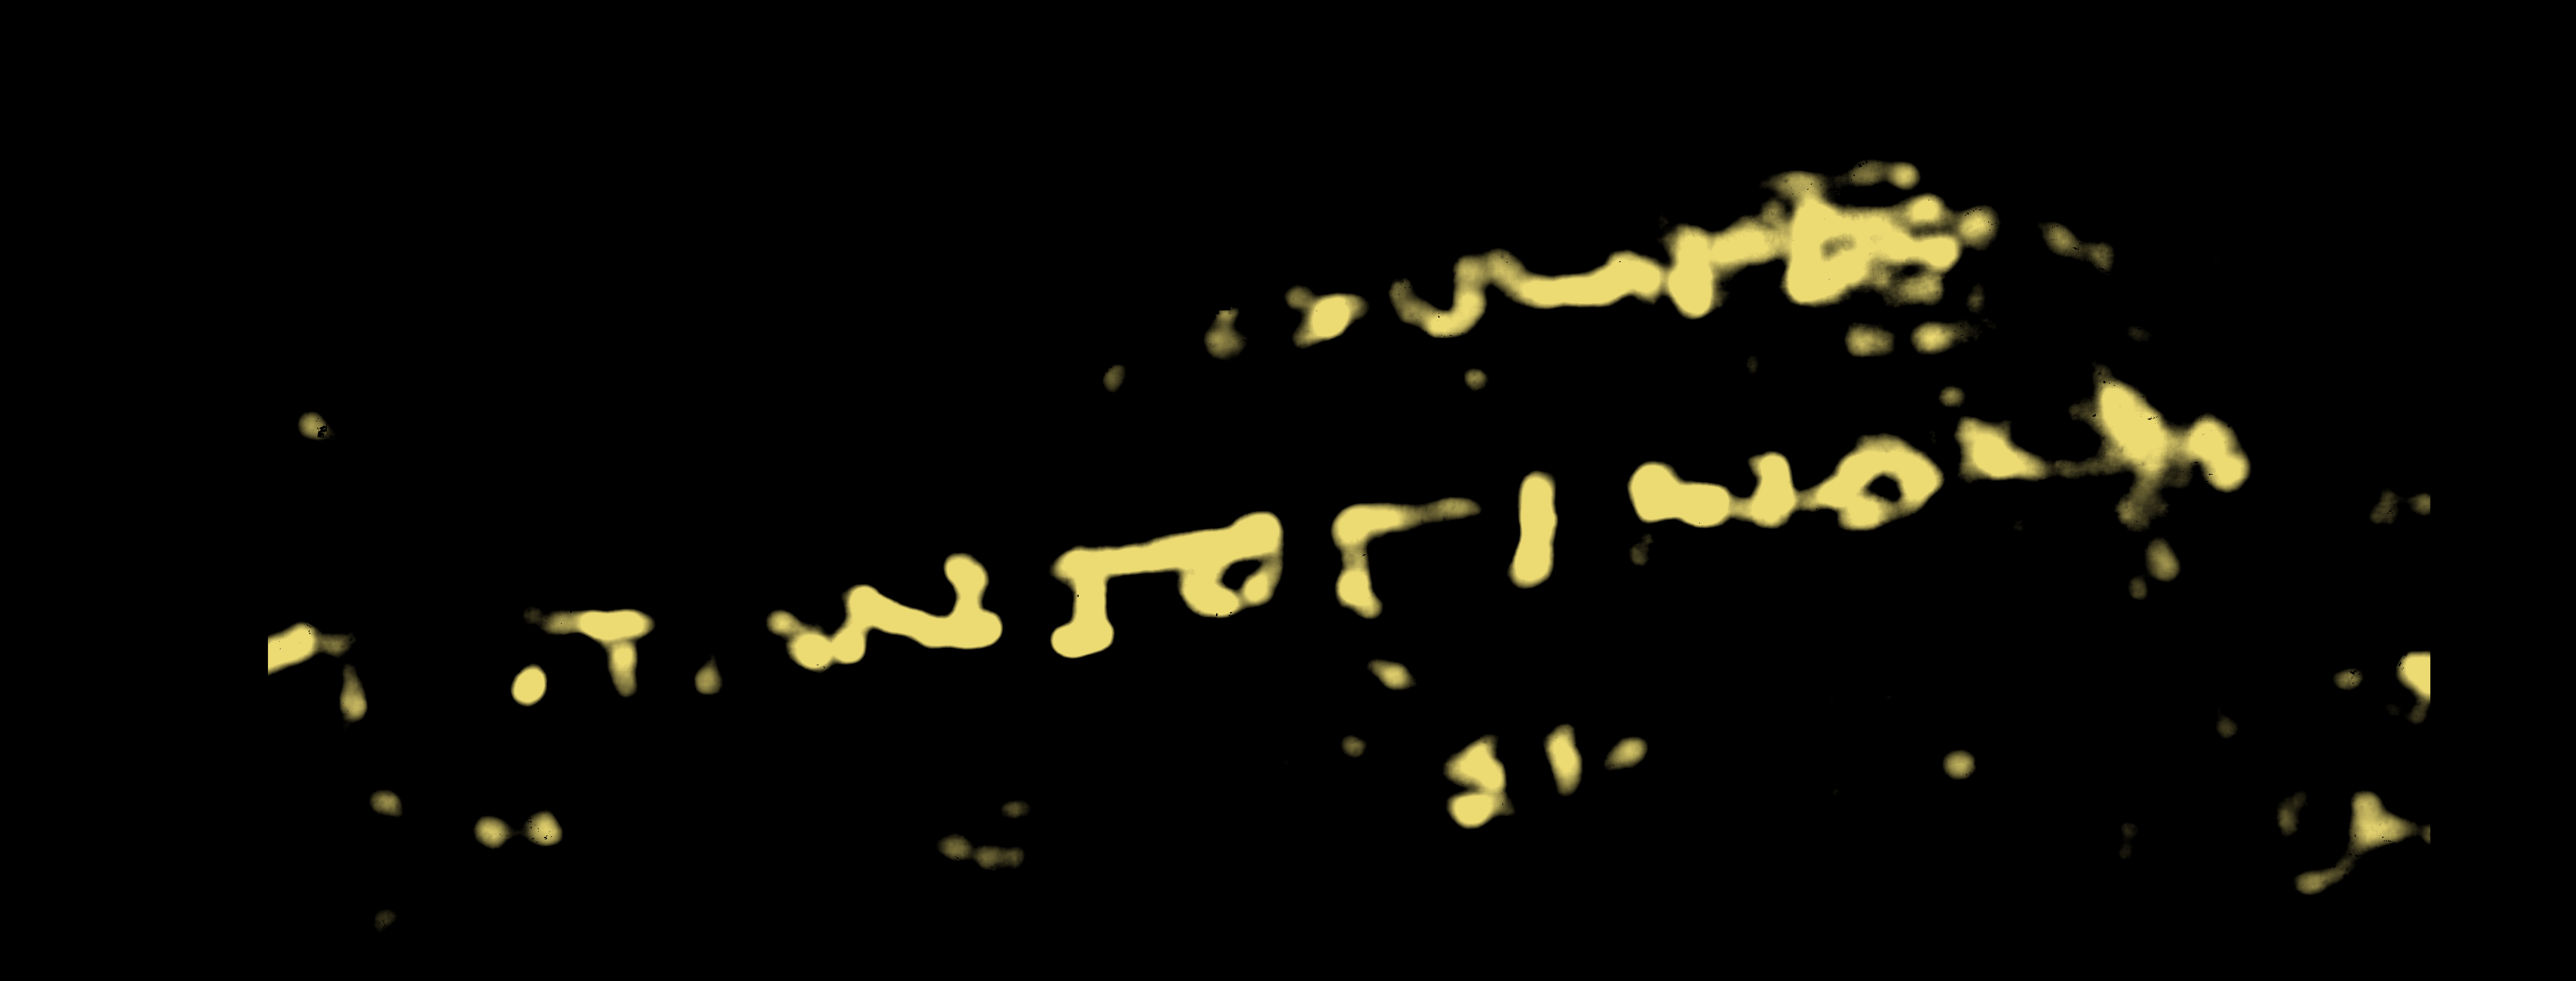
\includegraphics[width=0.29\textwidth]{../figures/m4/0343_1_reader-v3.png}
\hspace{3pt}
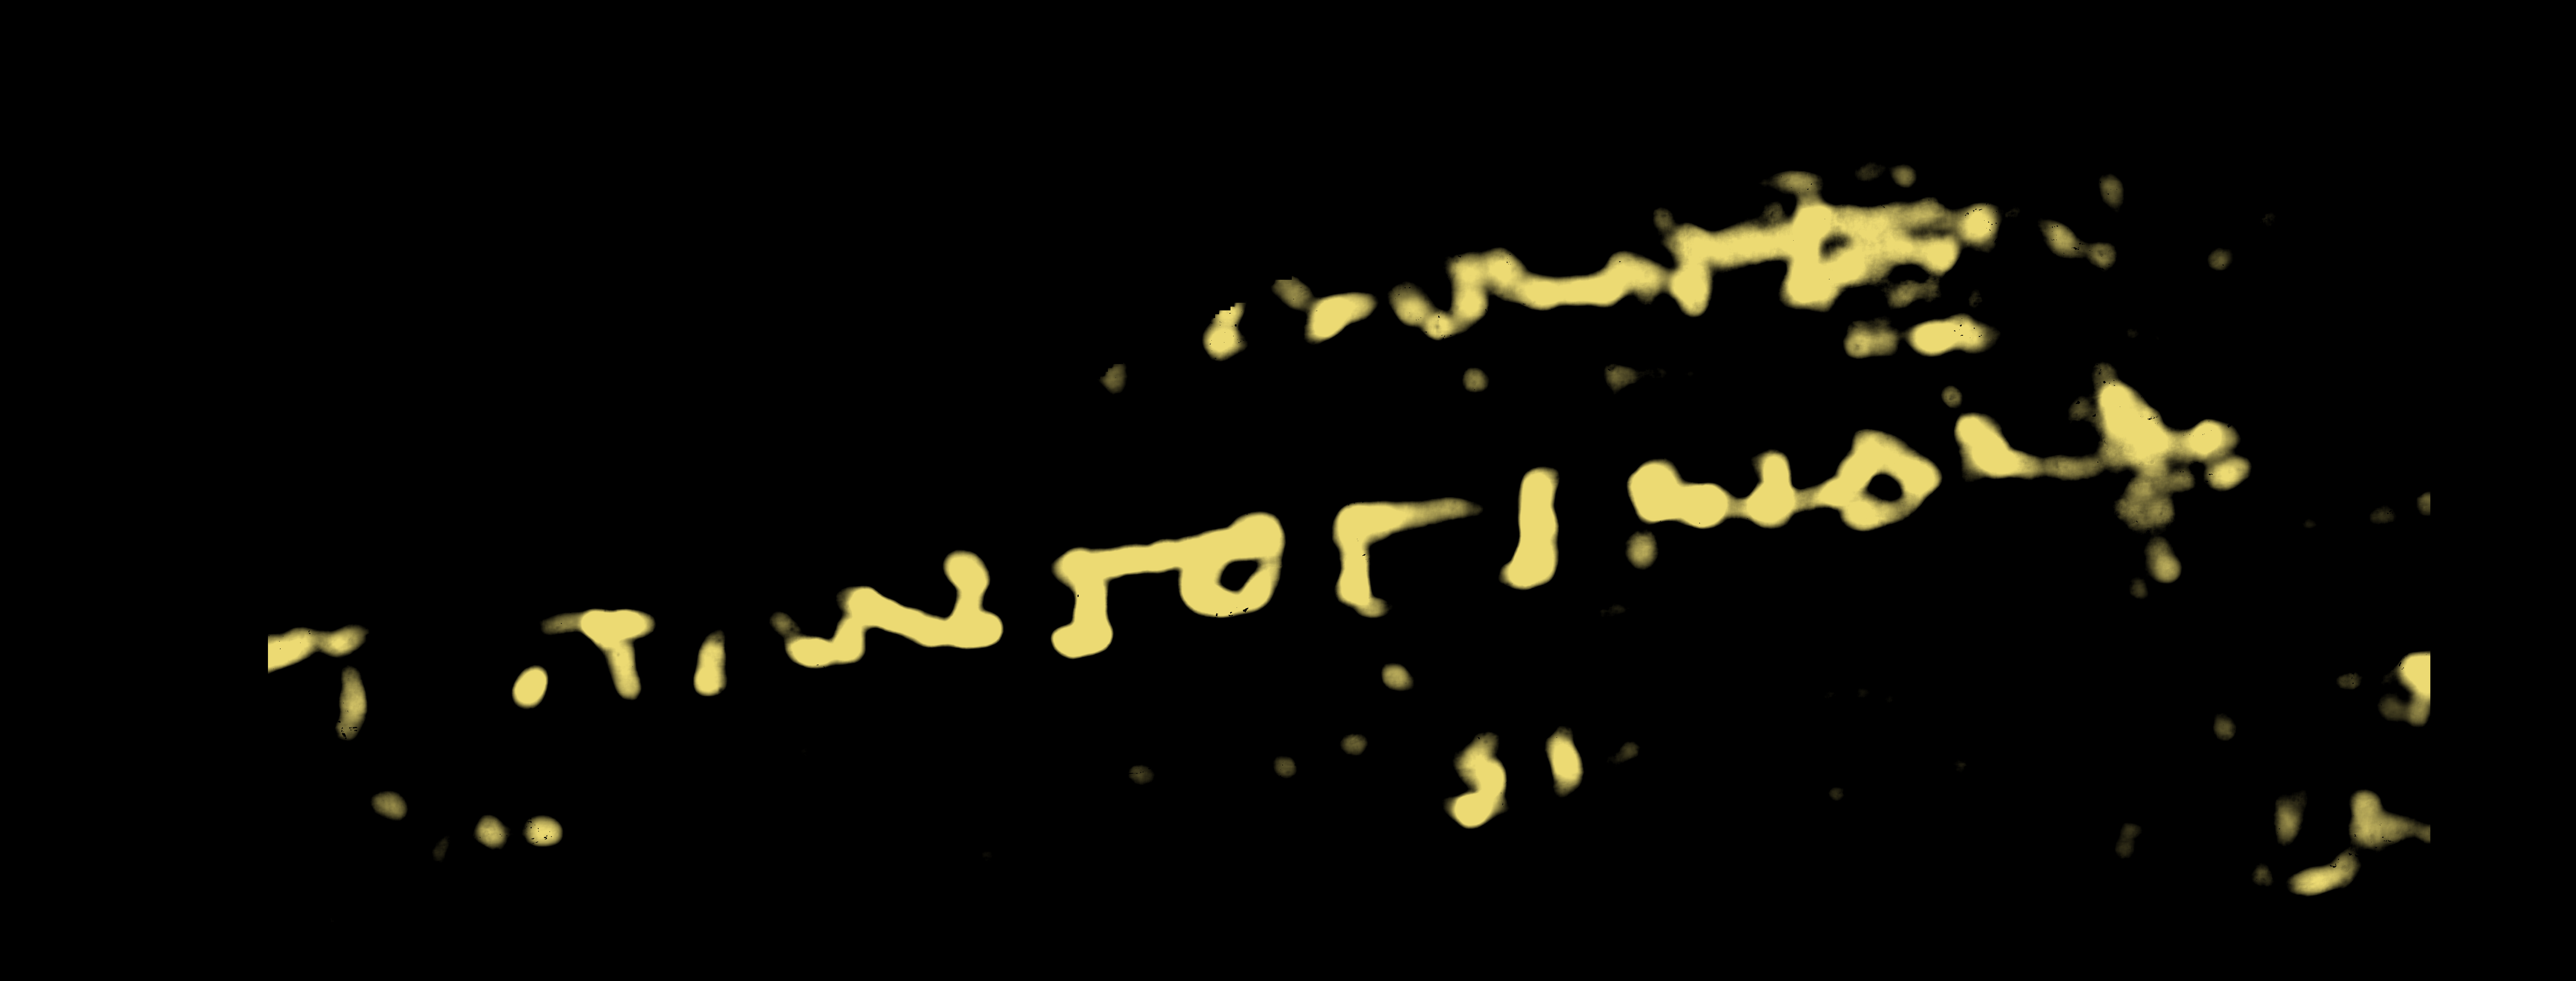
\includegraphics[width=0.29\textwidth]{../figures/m4/0343_2_m4.png}
\hspace{3pt}
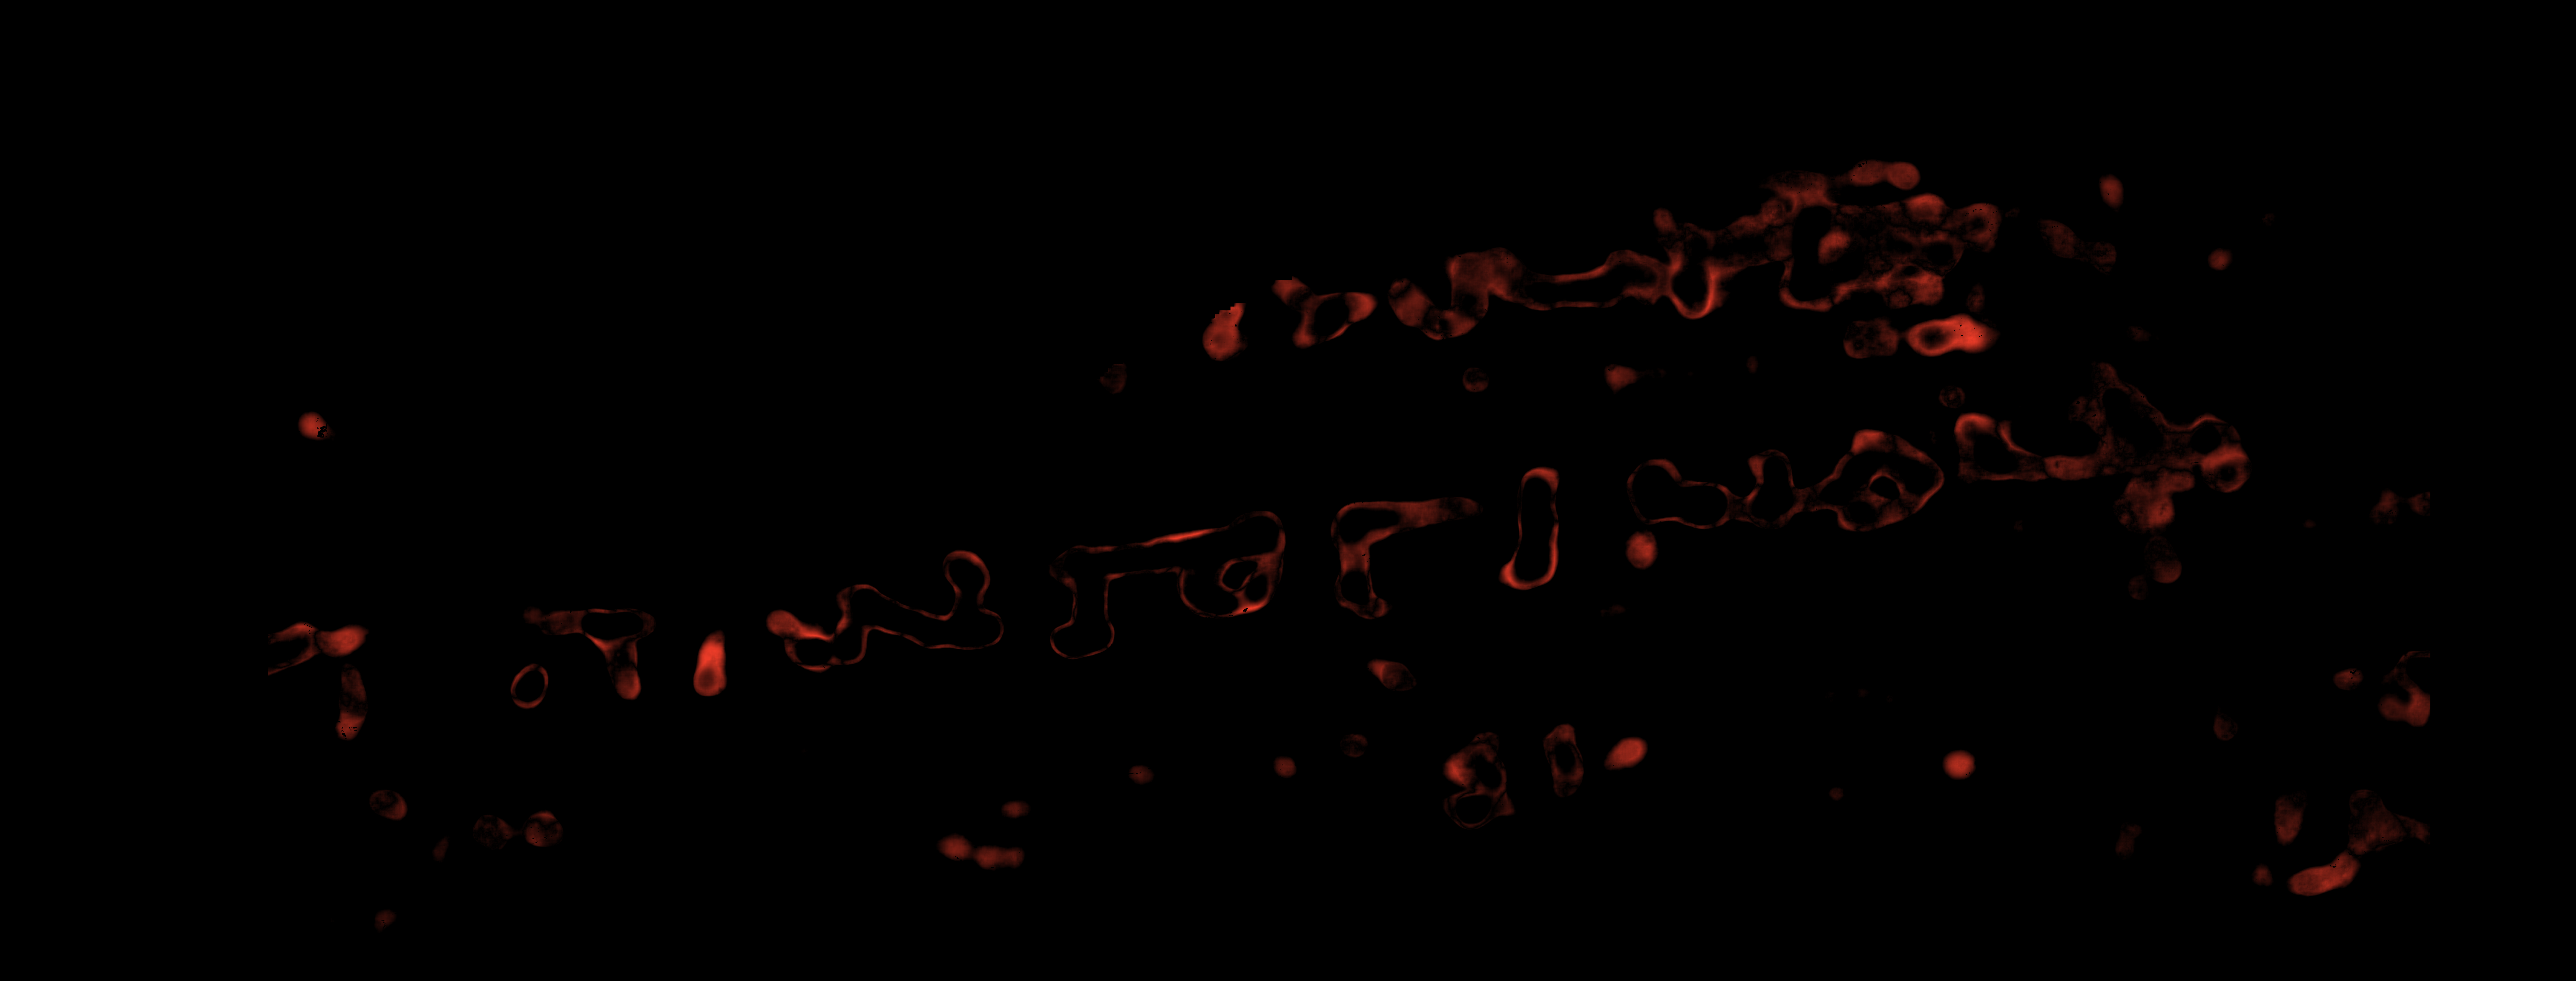
\includegraphics[width=0.29\textwidth]{../figures/m4/0343_3_difference.png}
\caption{Control unit 0343. Left, Reader v3 (AUC 0.9078); centre, \MfName{} (AUC 0.9064); right, the red difference between the two maps. Each map is stretched between its own percentiles, the panels are shown at the full resolution of the file.}\label{fig:m4-0343}
\end{figure*}

\begin{figure*}[!tp]
\centering
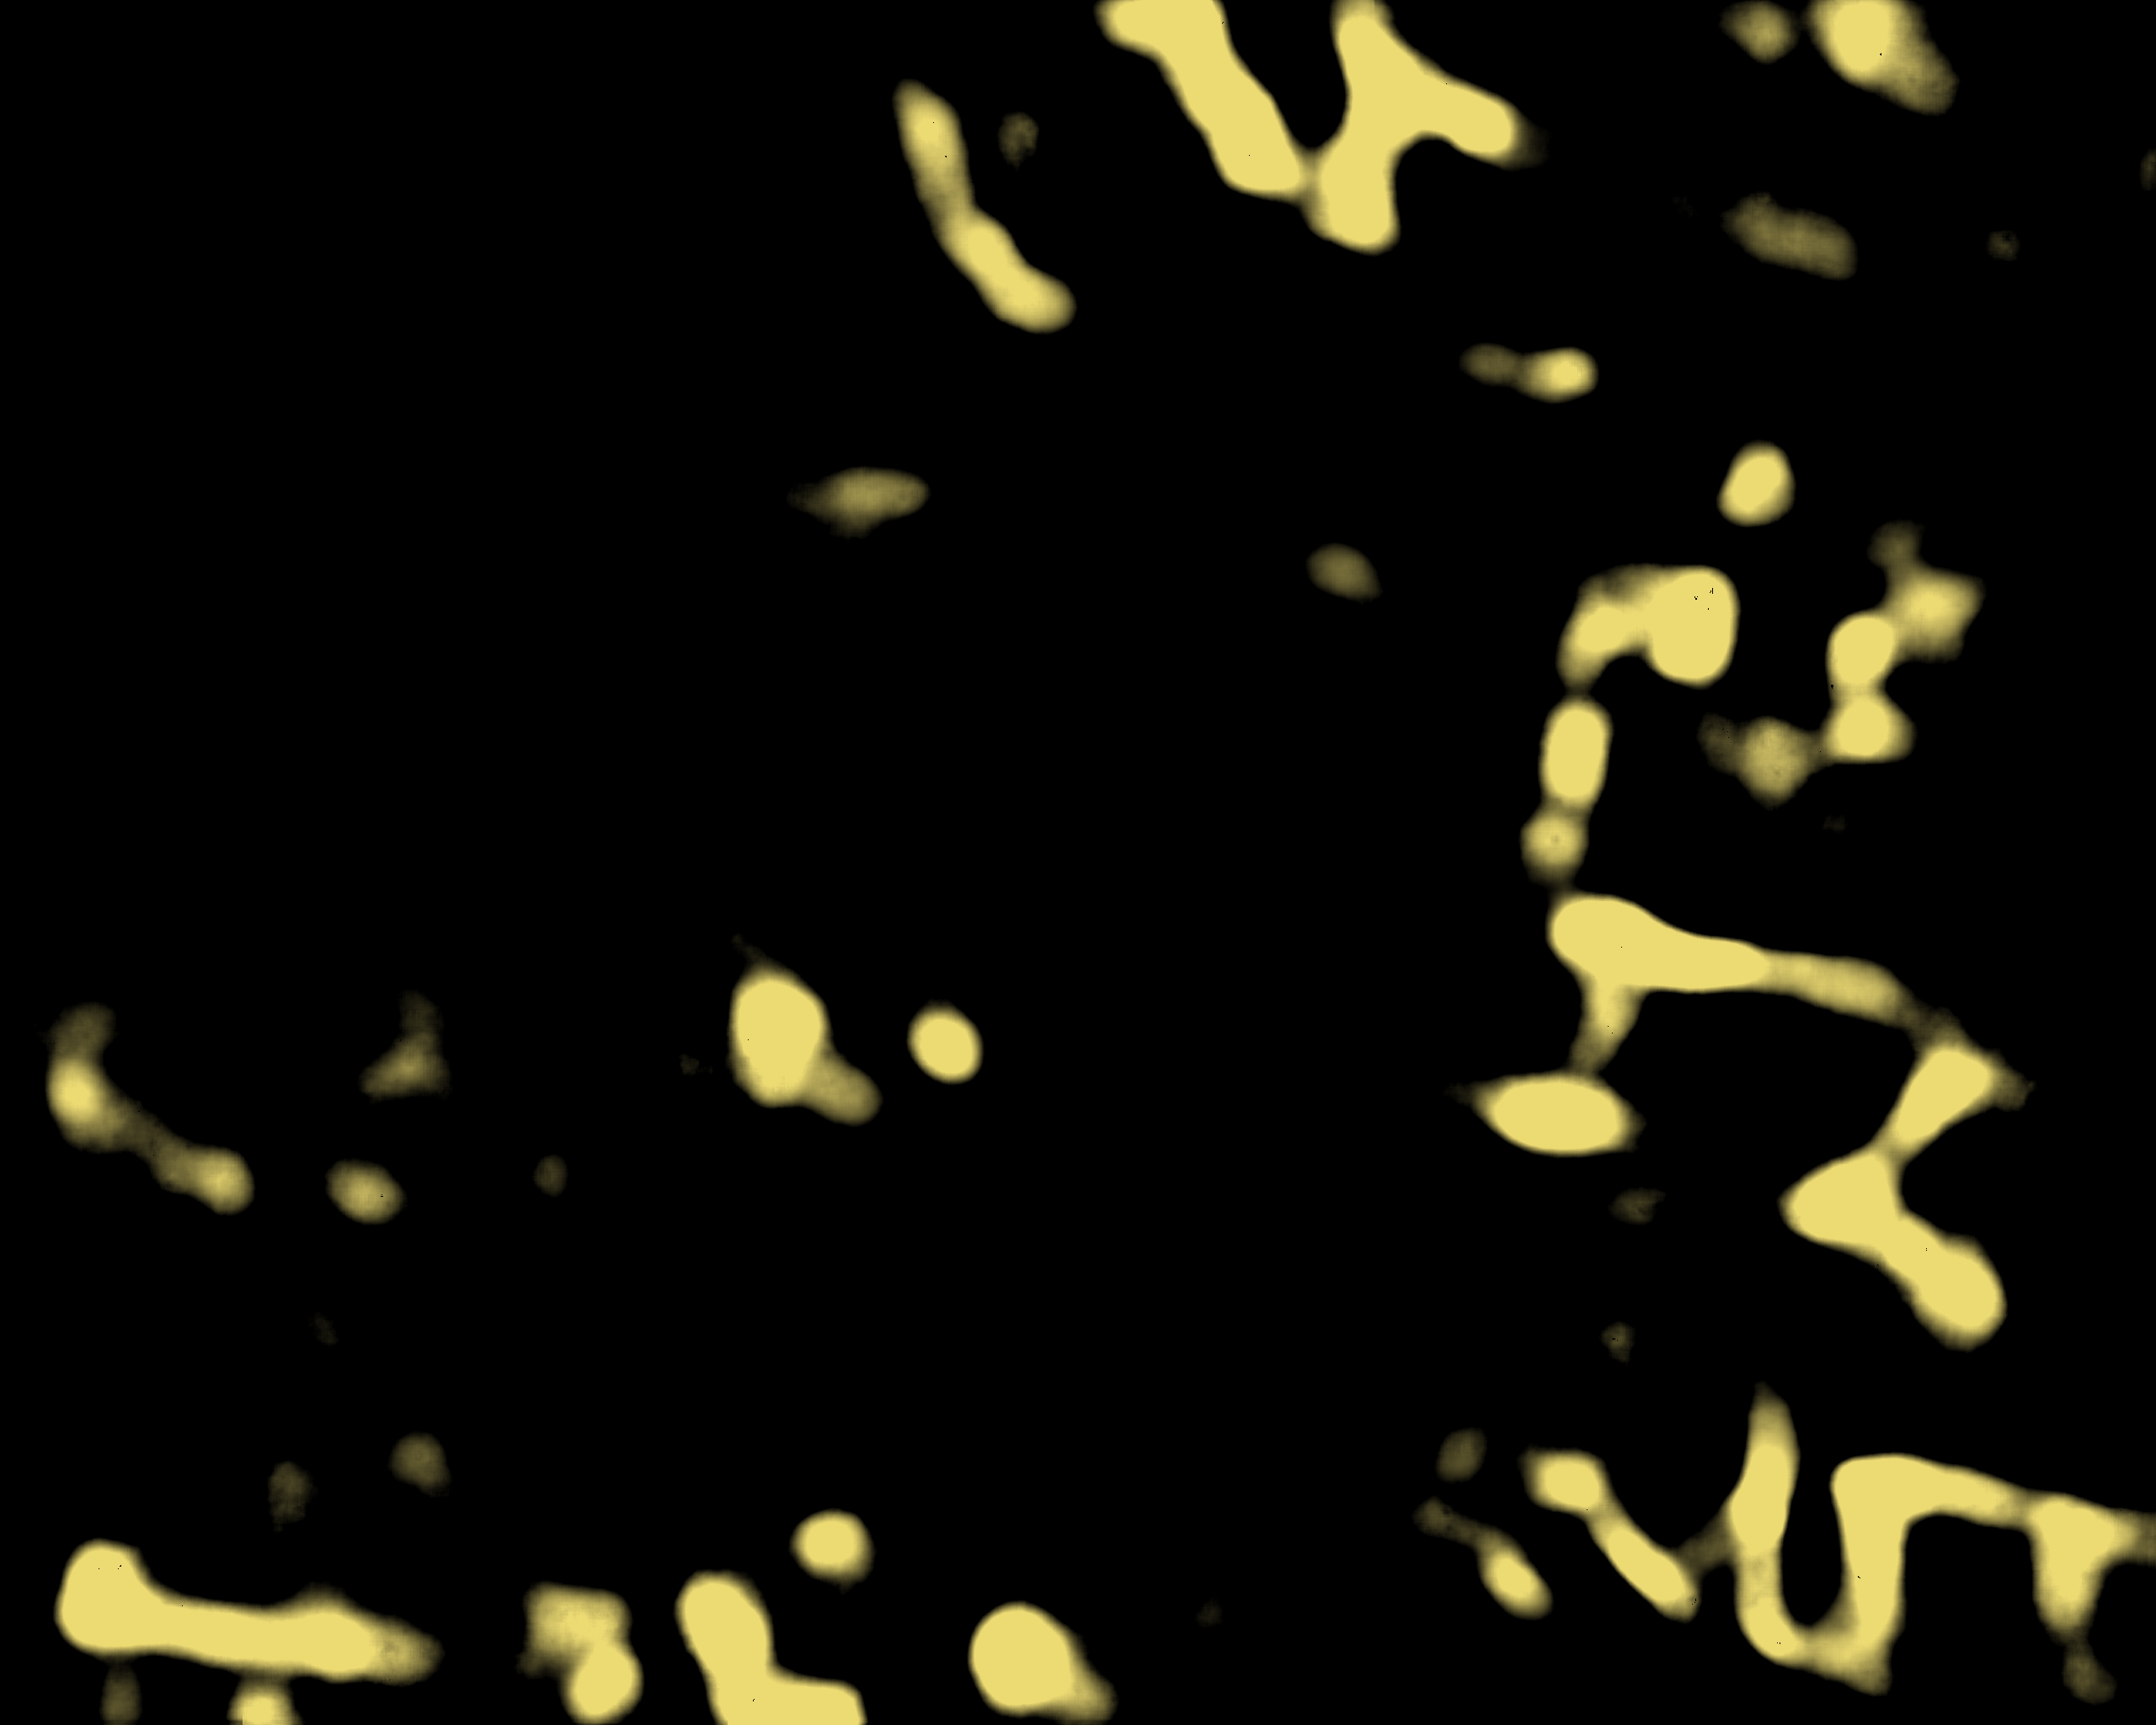
\includegraphics[width=0.29\textwidth]{../figures/m4/ag1_1_reader-v3.png}
\hspace{3pt}
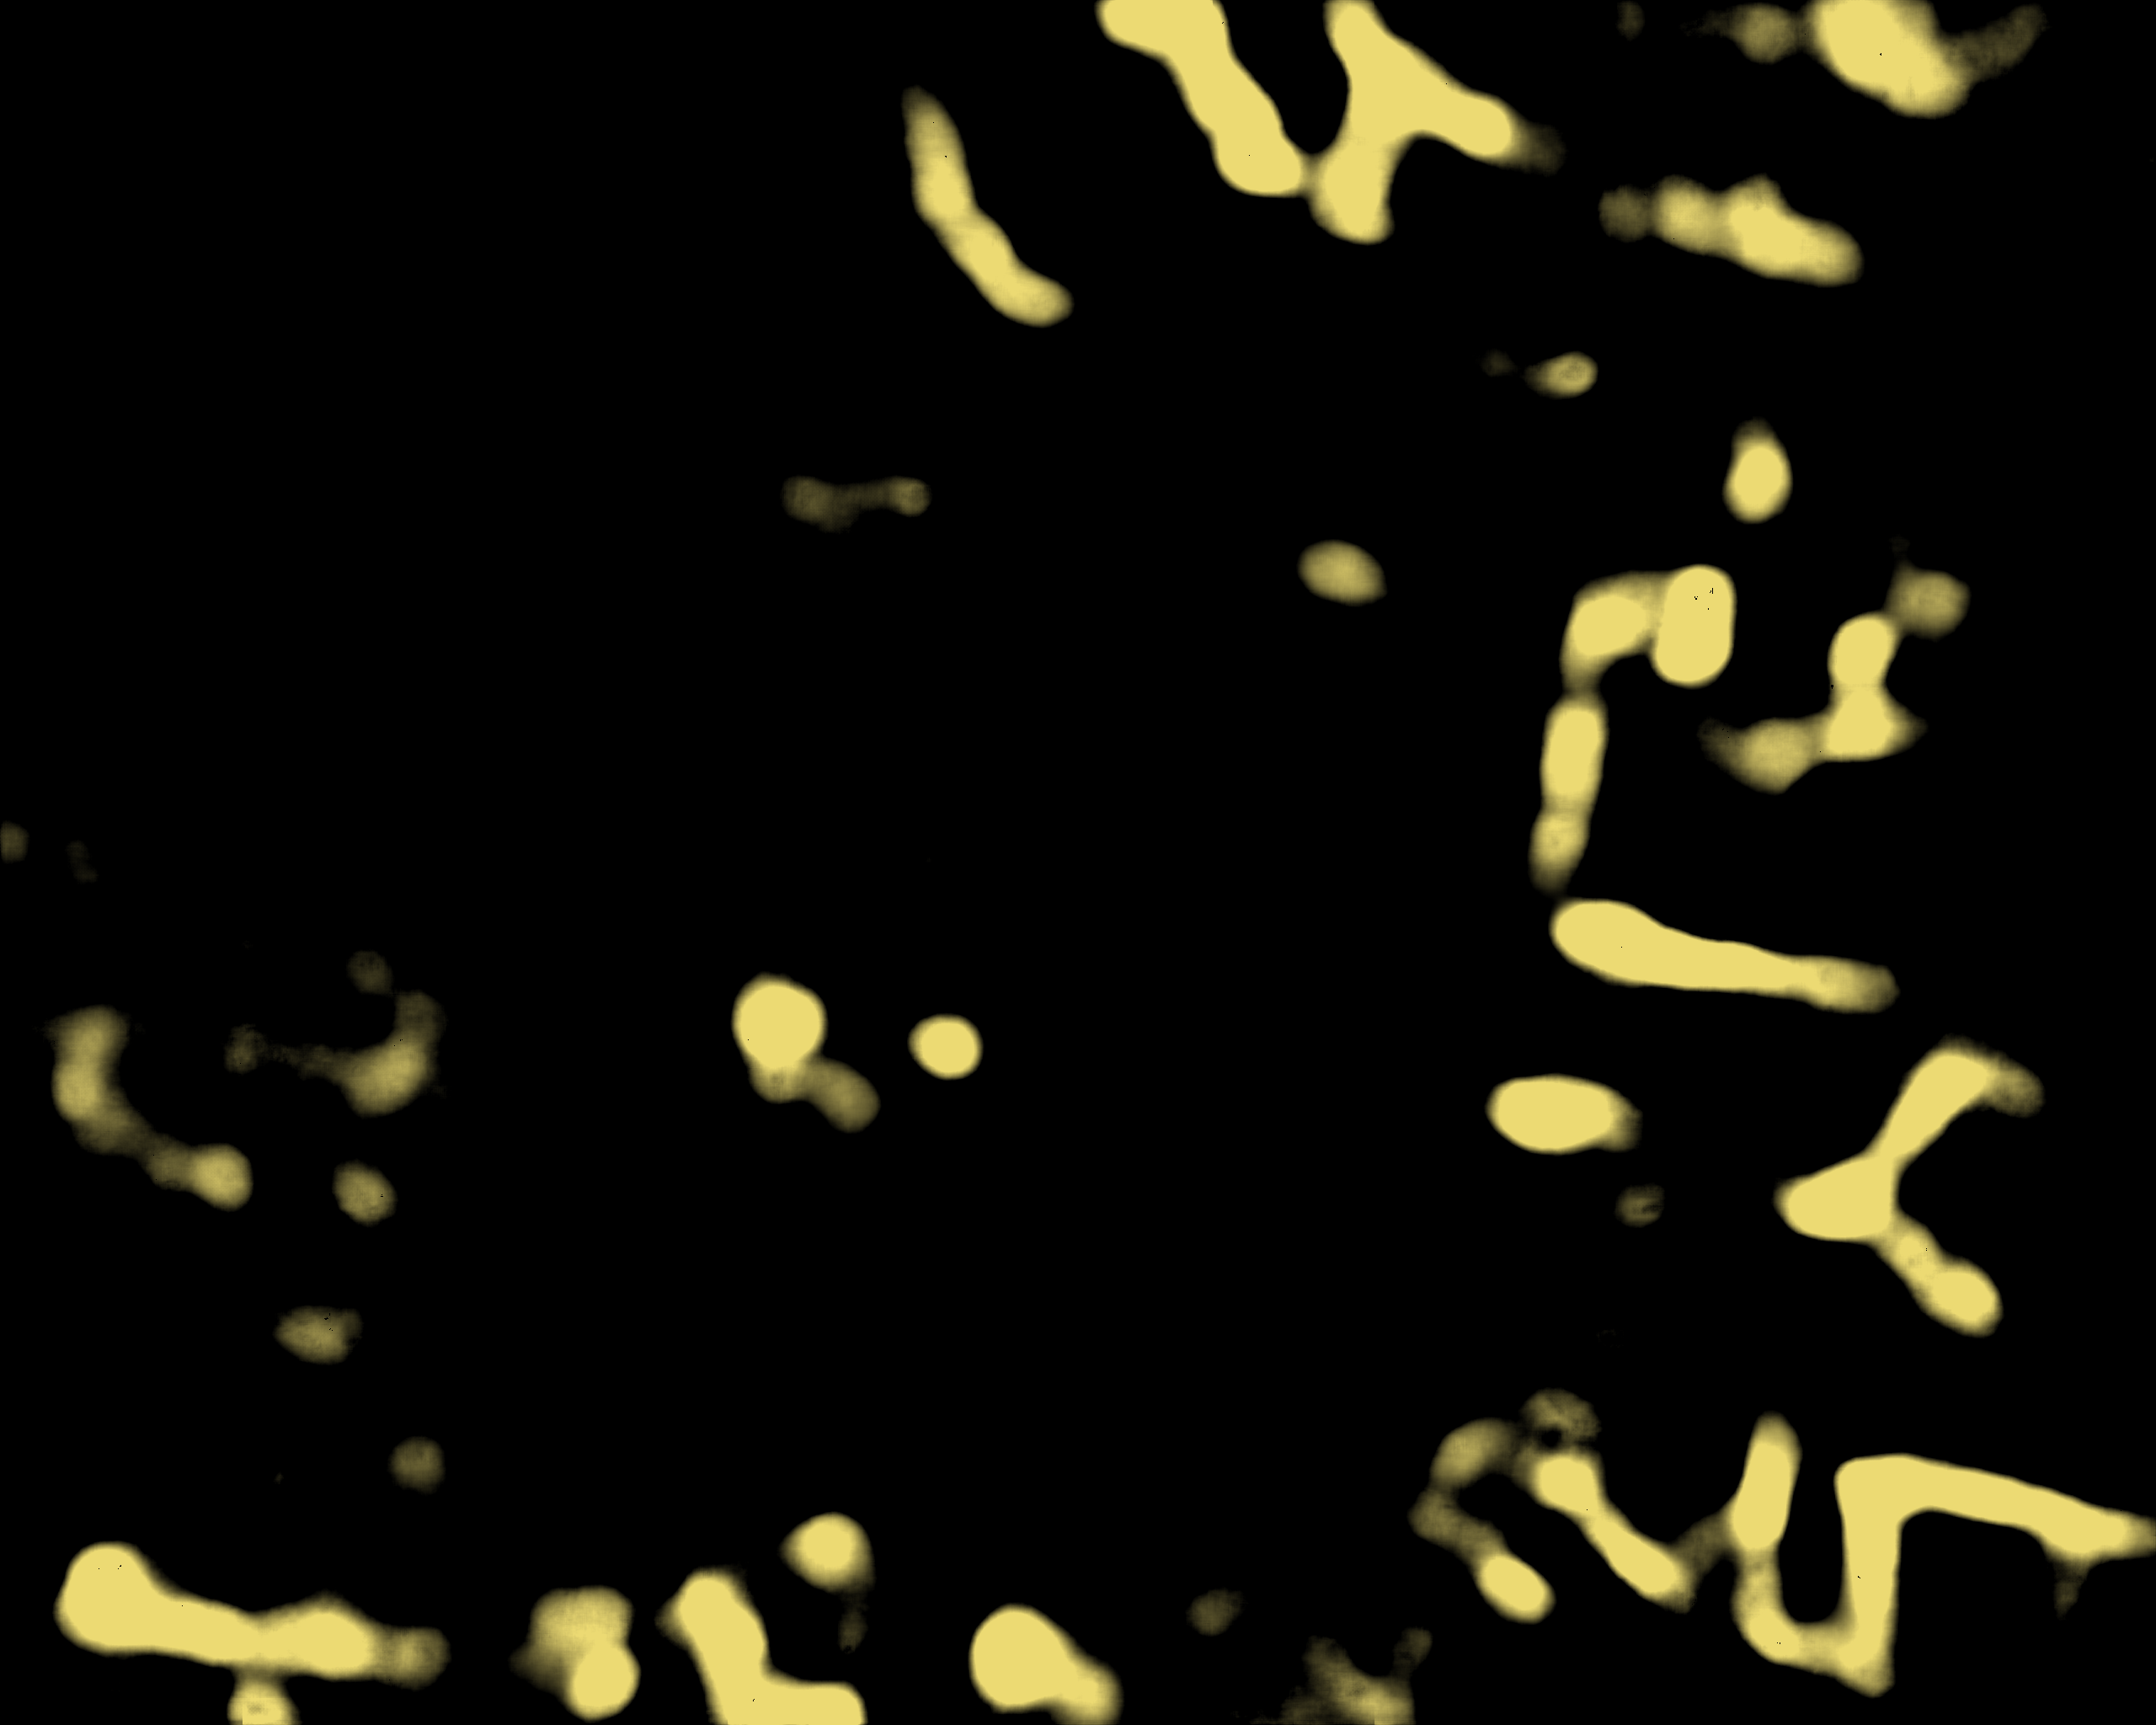
\includegraphics[width=0.29\textwidth]{../figures/m4/ag1_2_m4.png}
\hspace{3pt}
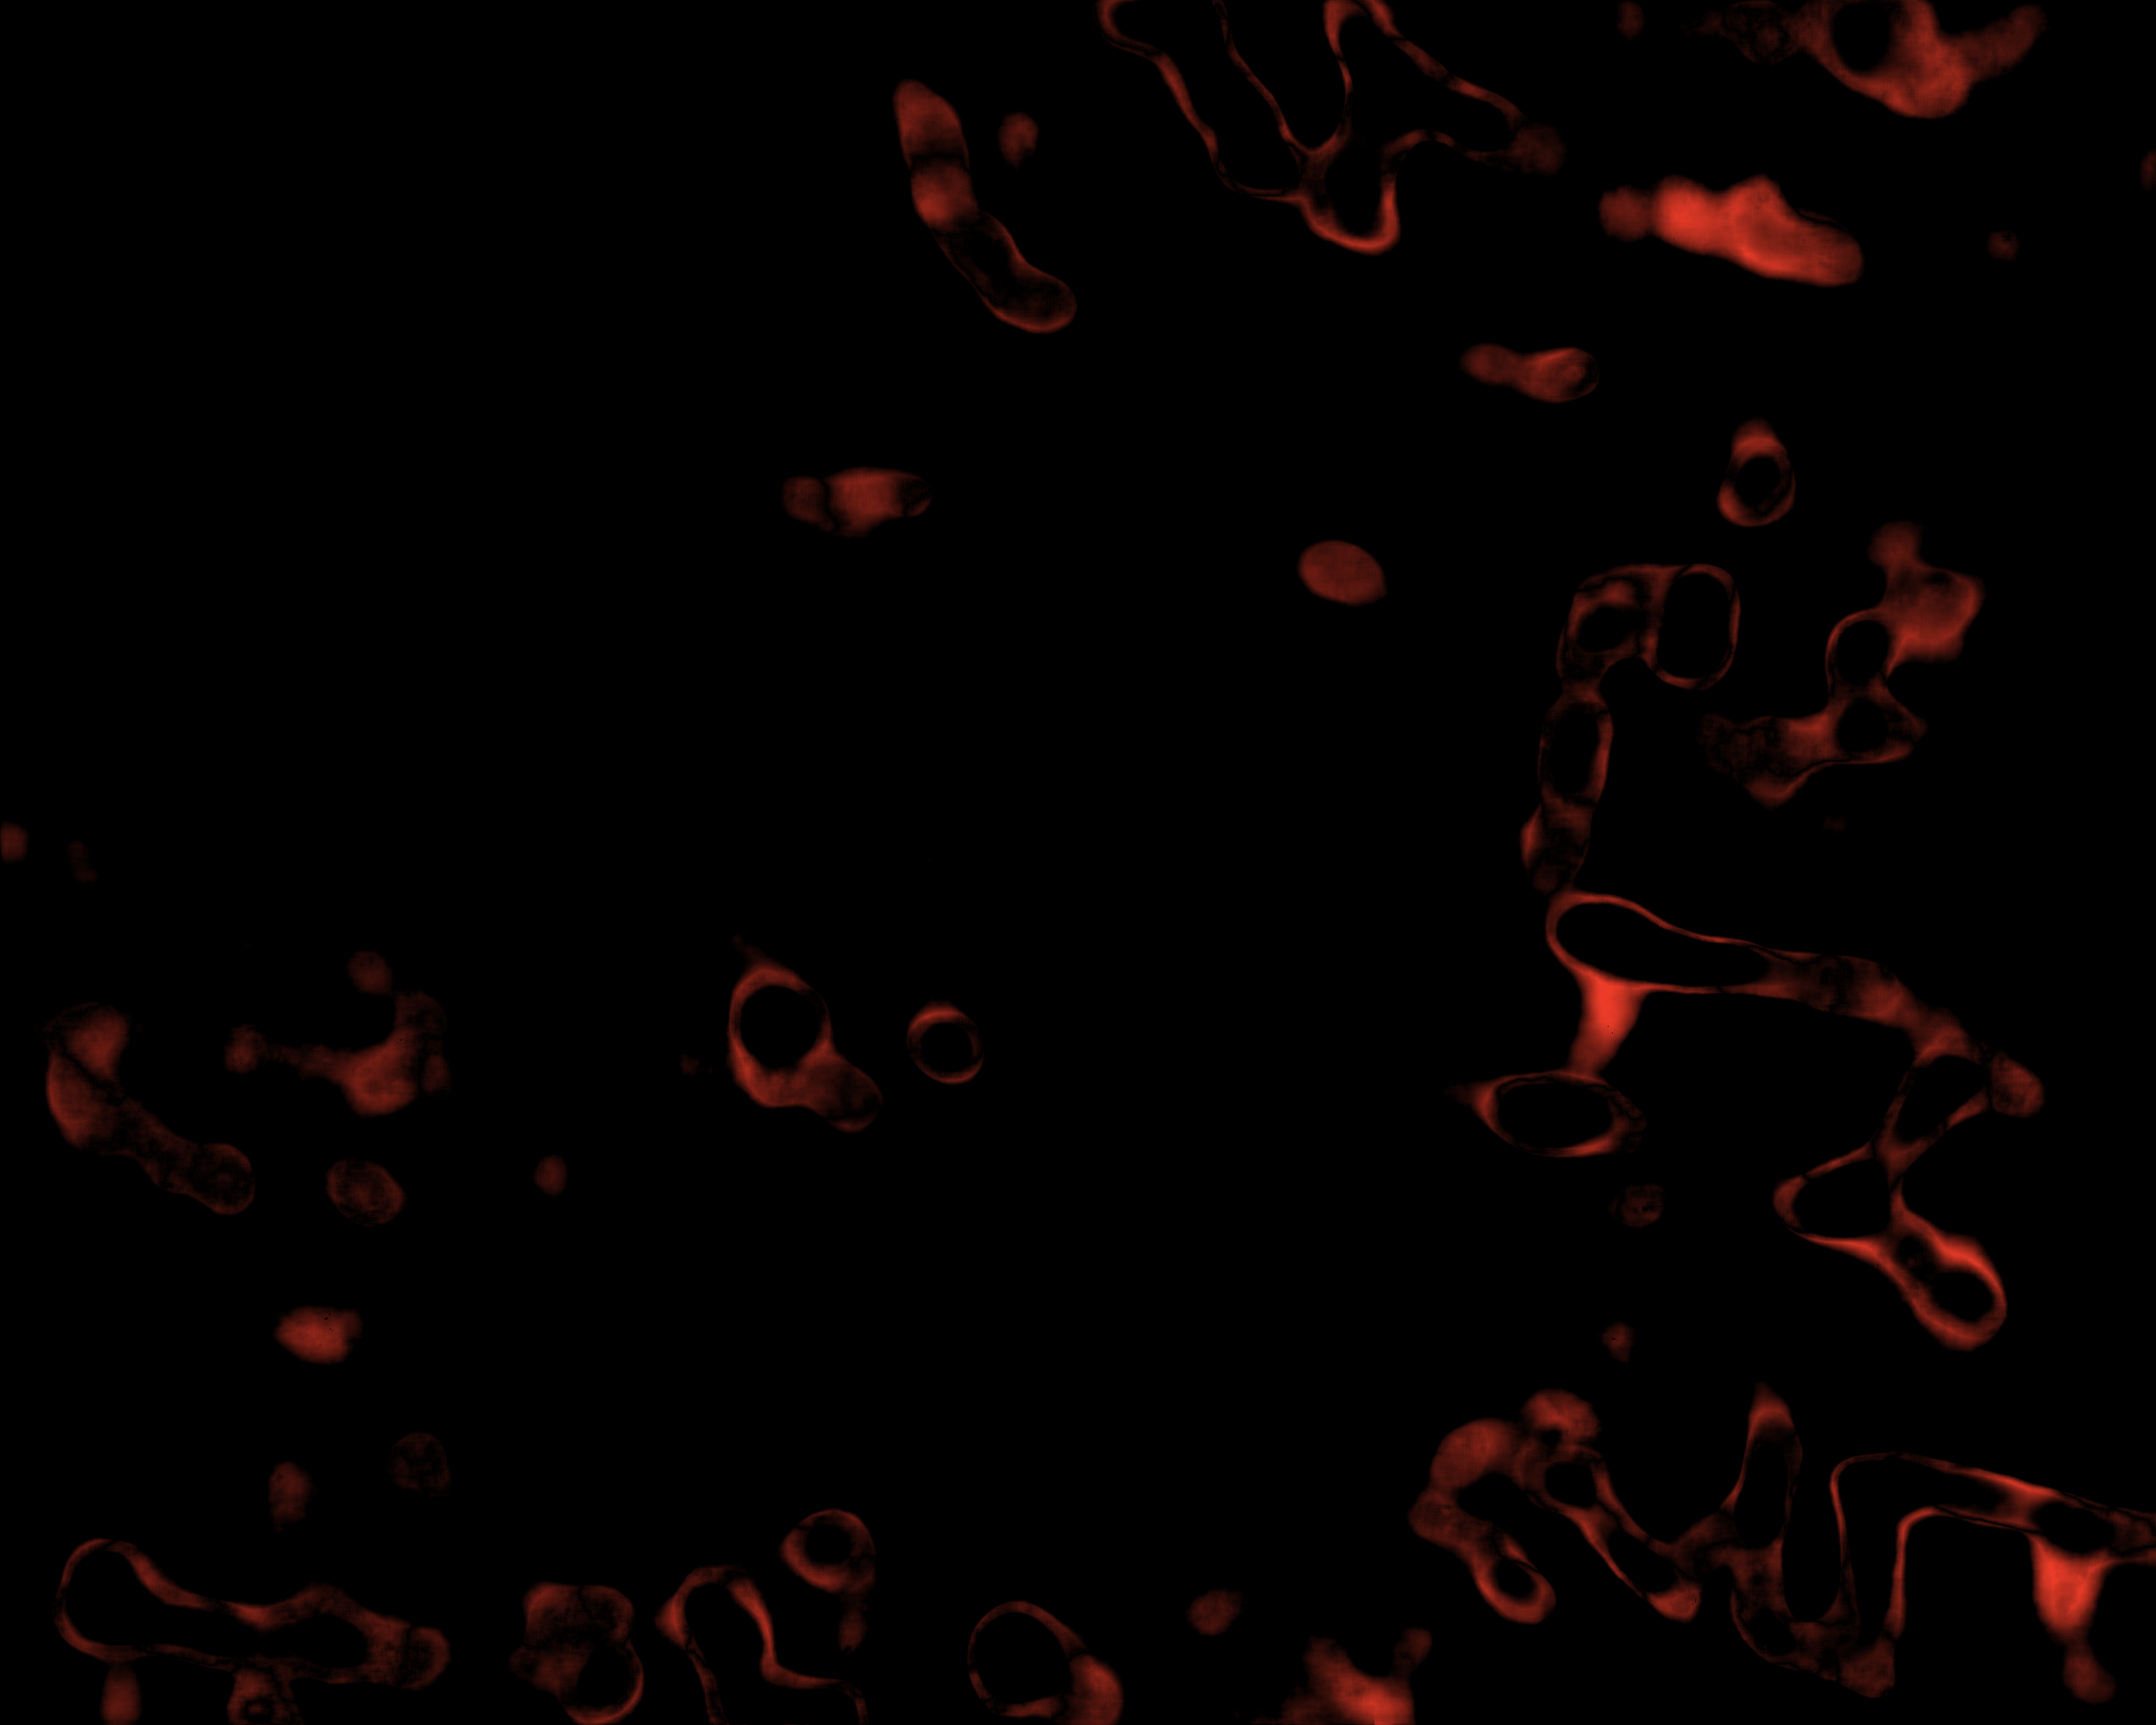
\includegraphics[width=0.29\textwidth]{../figures/m4/ag1_3_difference.png}
\caption{Control unit 0841 ag1. Left, Reader v3 (AUC 0.8513); centre, \MfName{} (AUC 0.8598); right, the red difference between the two maps. Each map is stretched between its own percentiles, the panels are shown at the full resolution of the file.}\label{fig:m4-ag1}
\end{figure*}

\begin{figure*}[!tp]
\centering
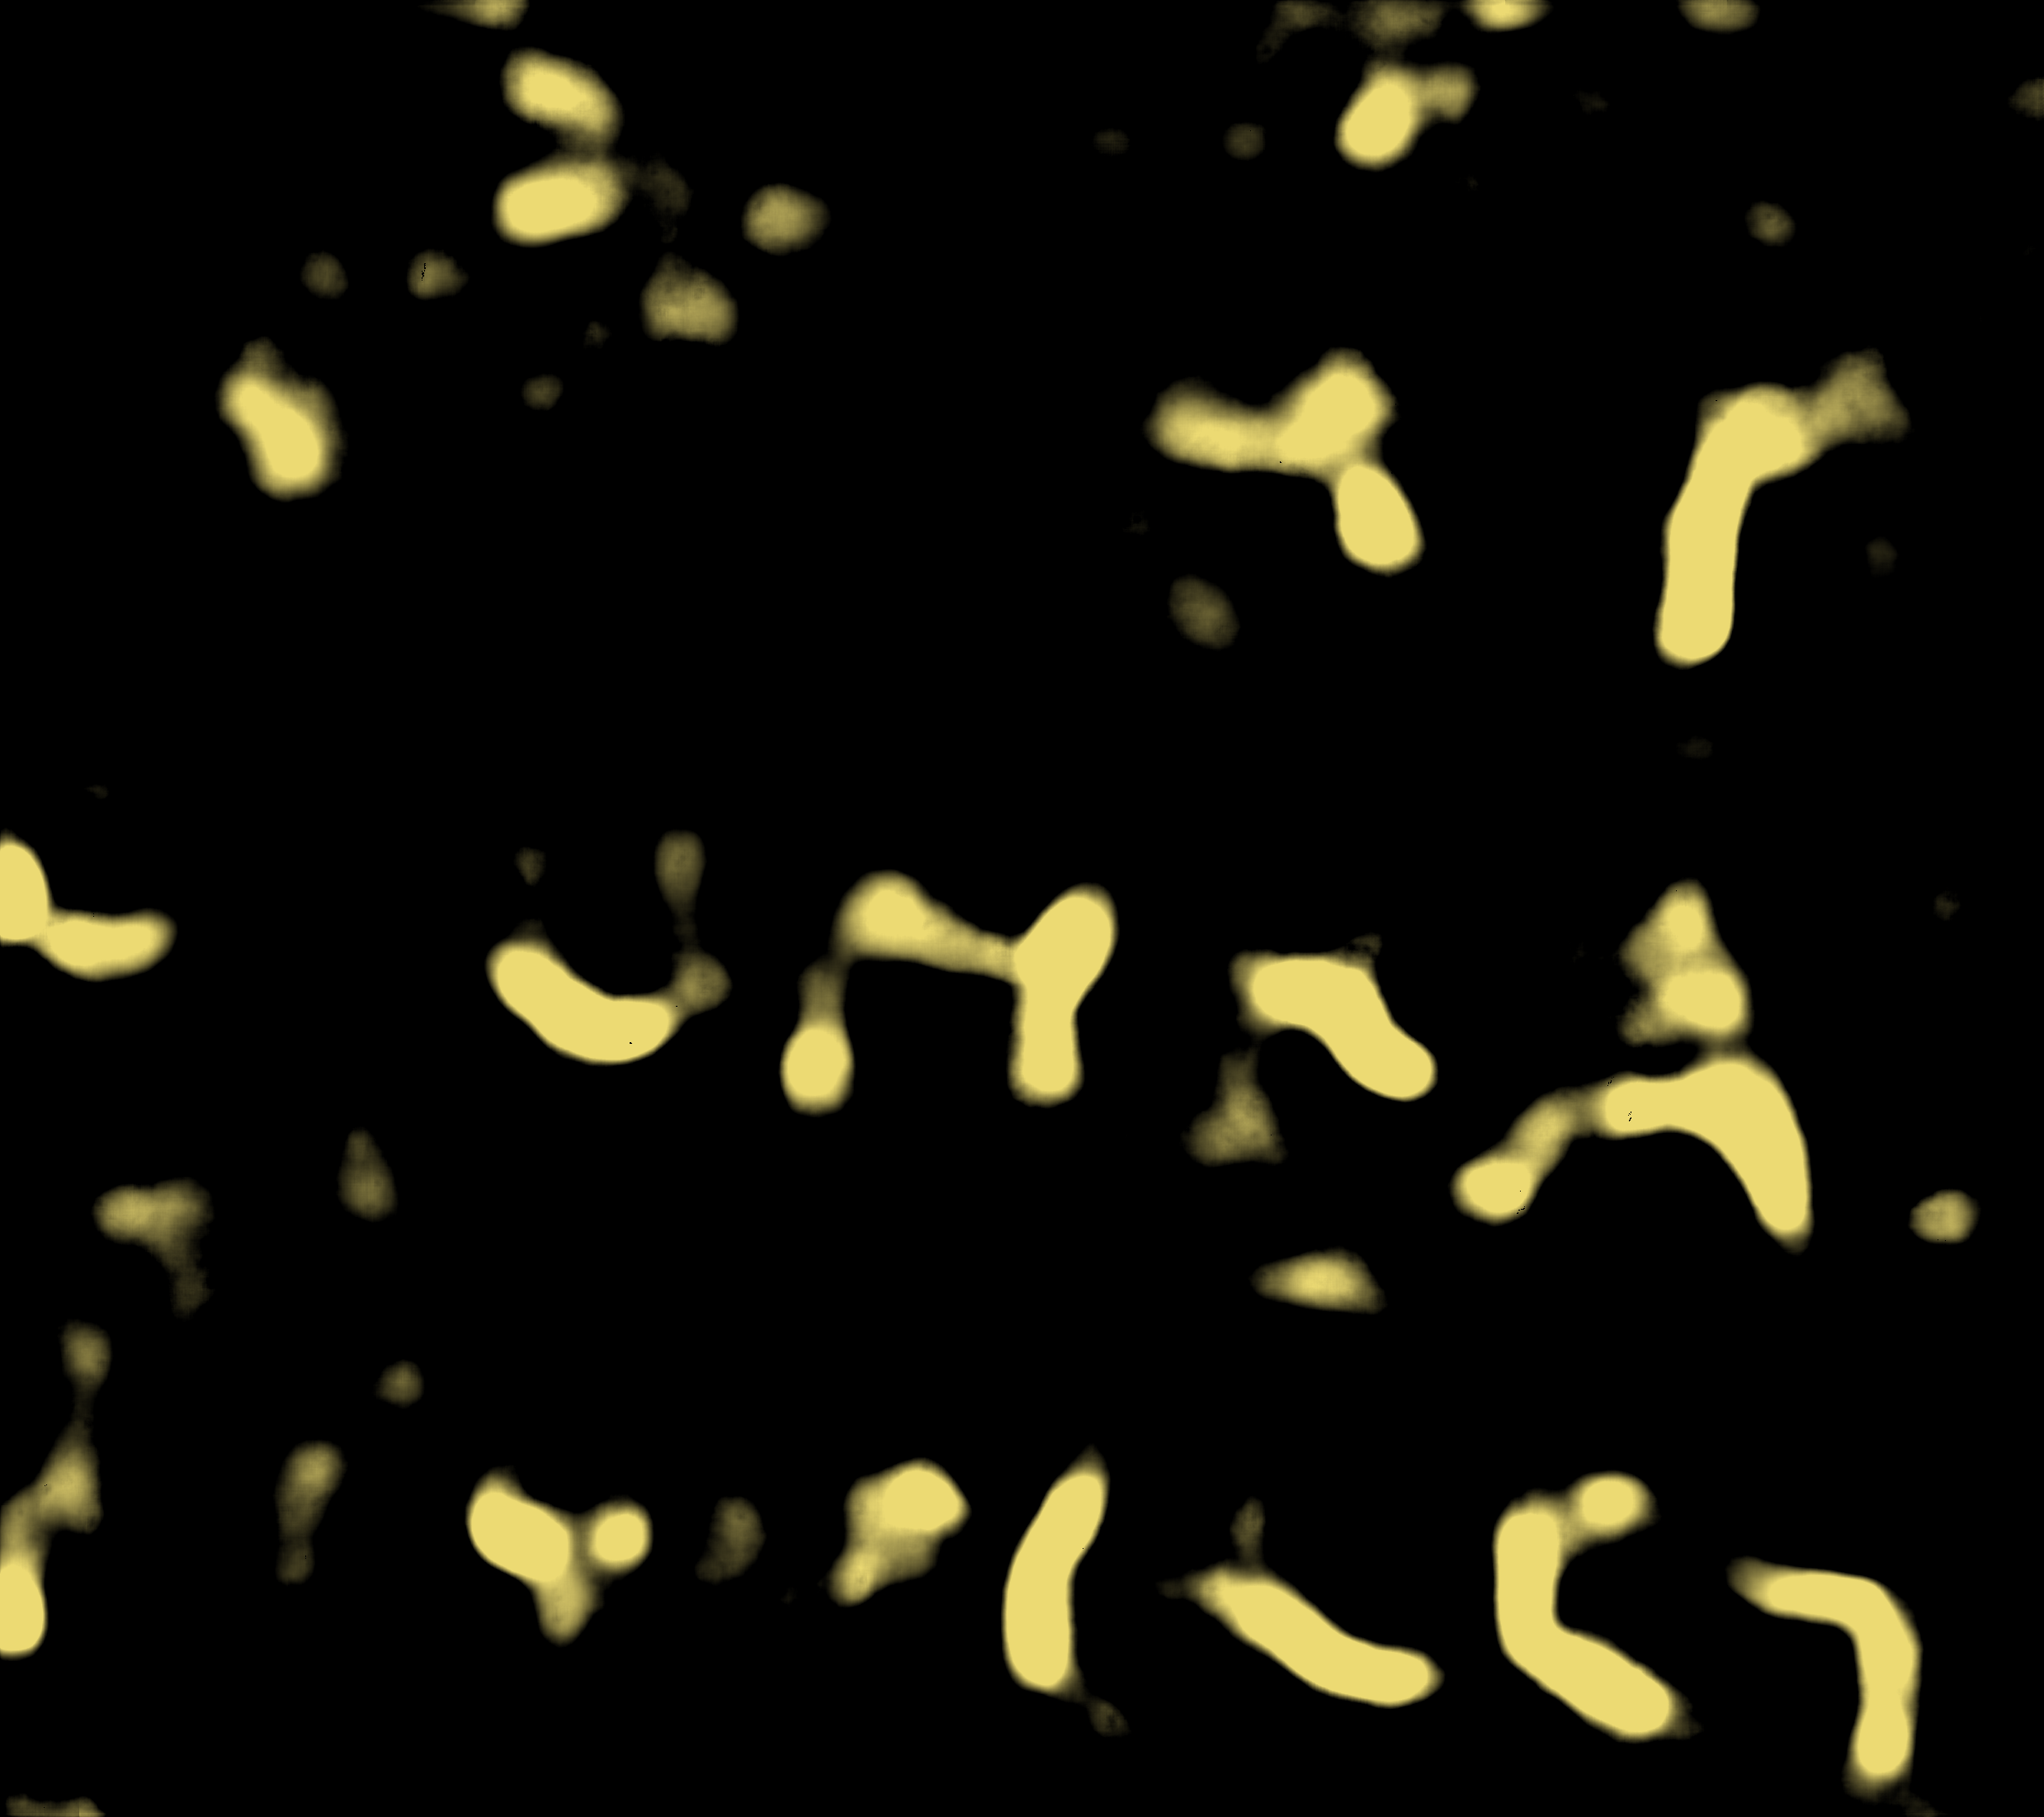
\includegraphics[width=0.29\textwidth]{../figures/m4/ag2_1_reader-v3.png}
\hspace{3pt}
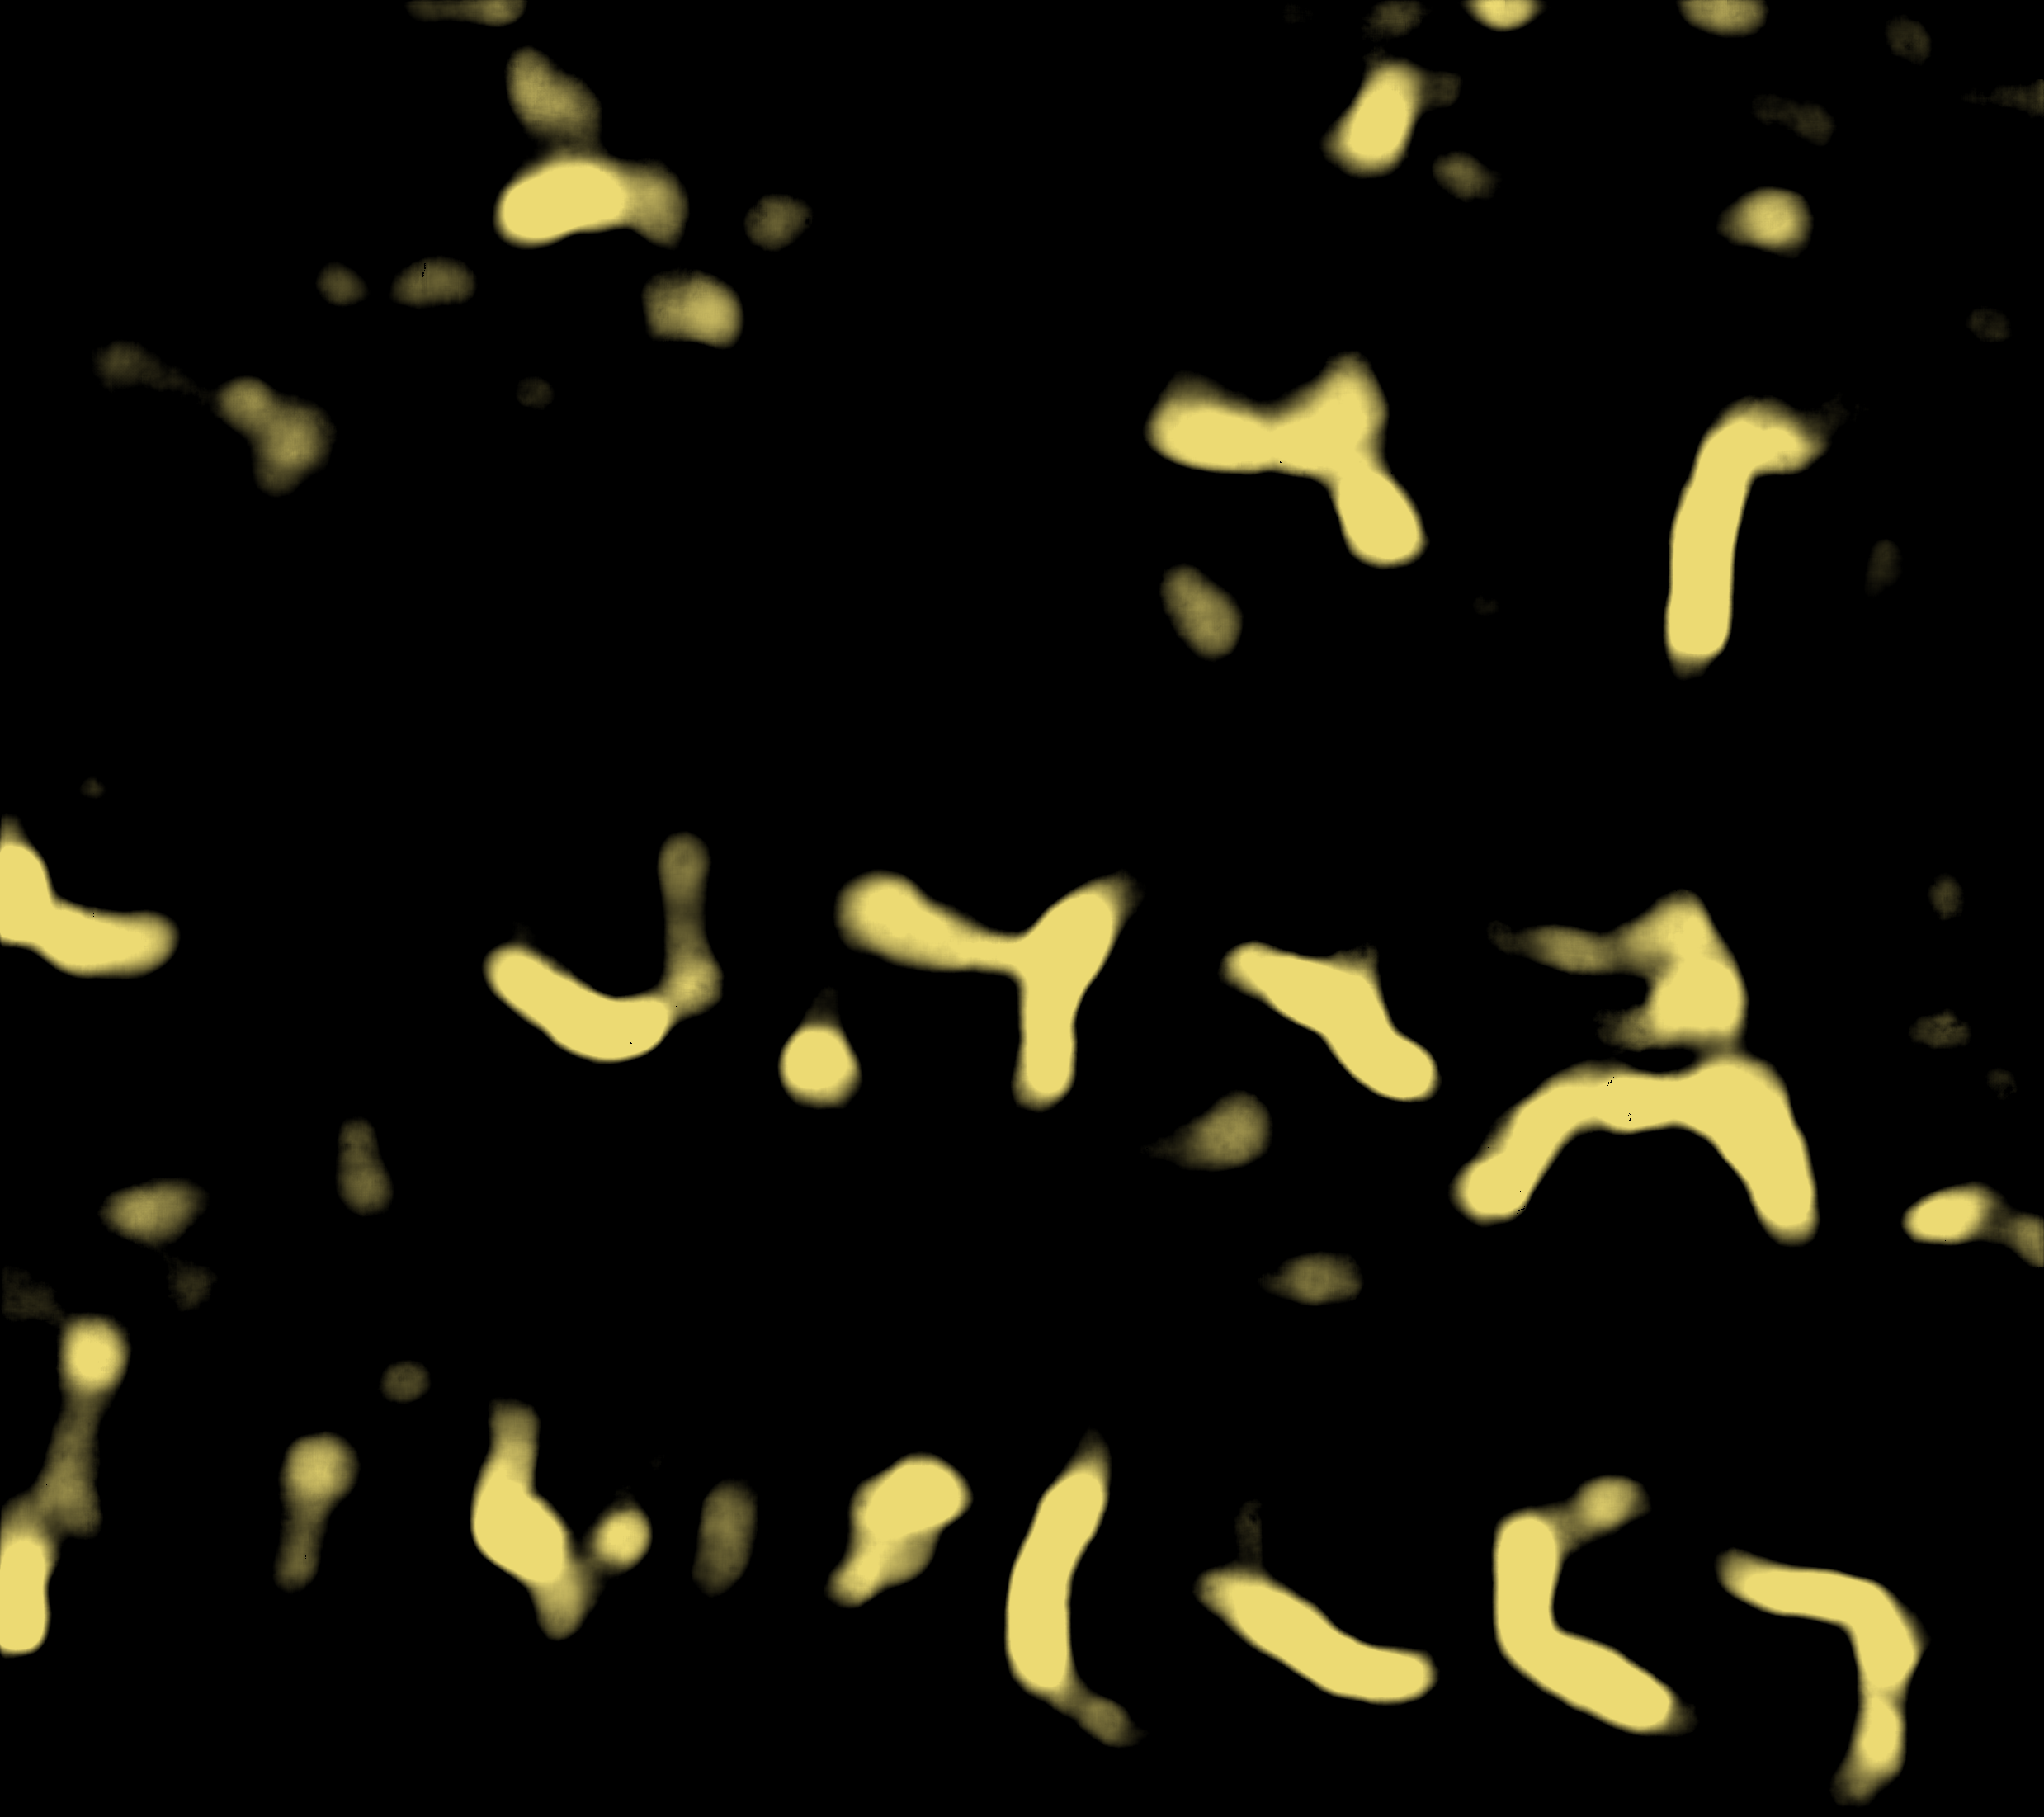
\includegraphics[width=0.29\textwidth]{../figures/m4/ag2_2_m4.png}
\hspace{3pt}
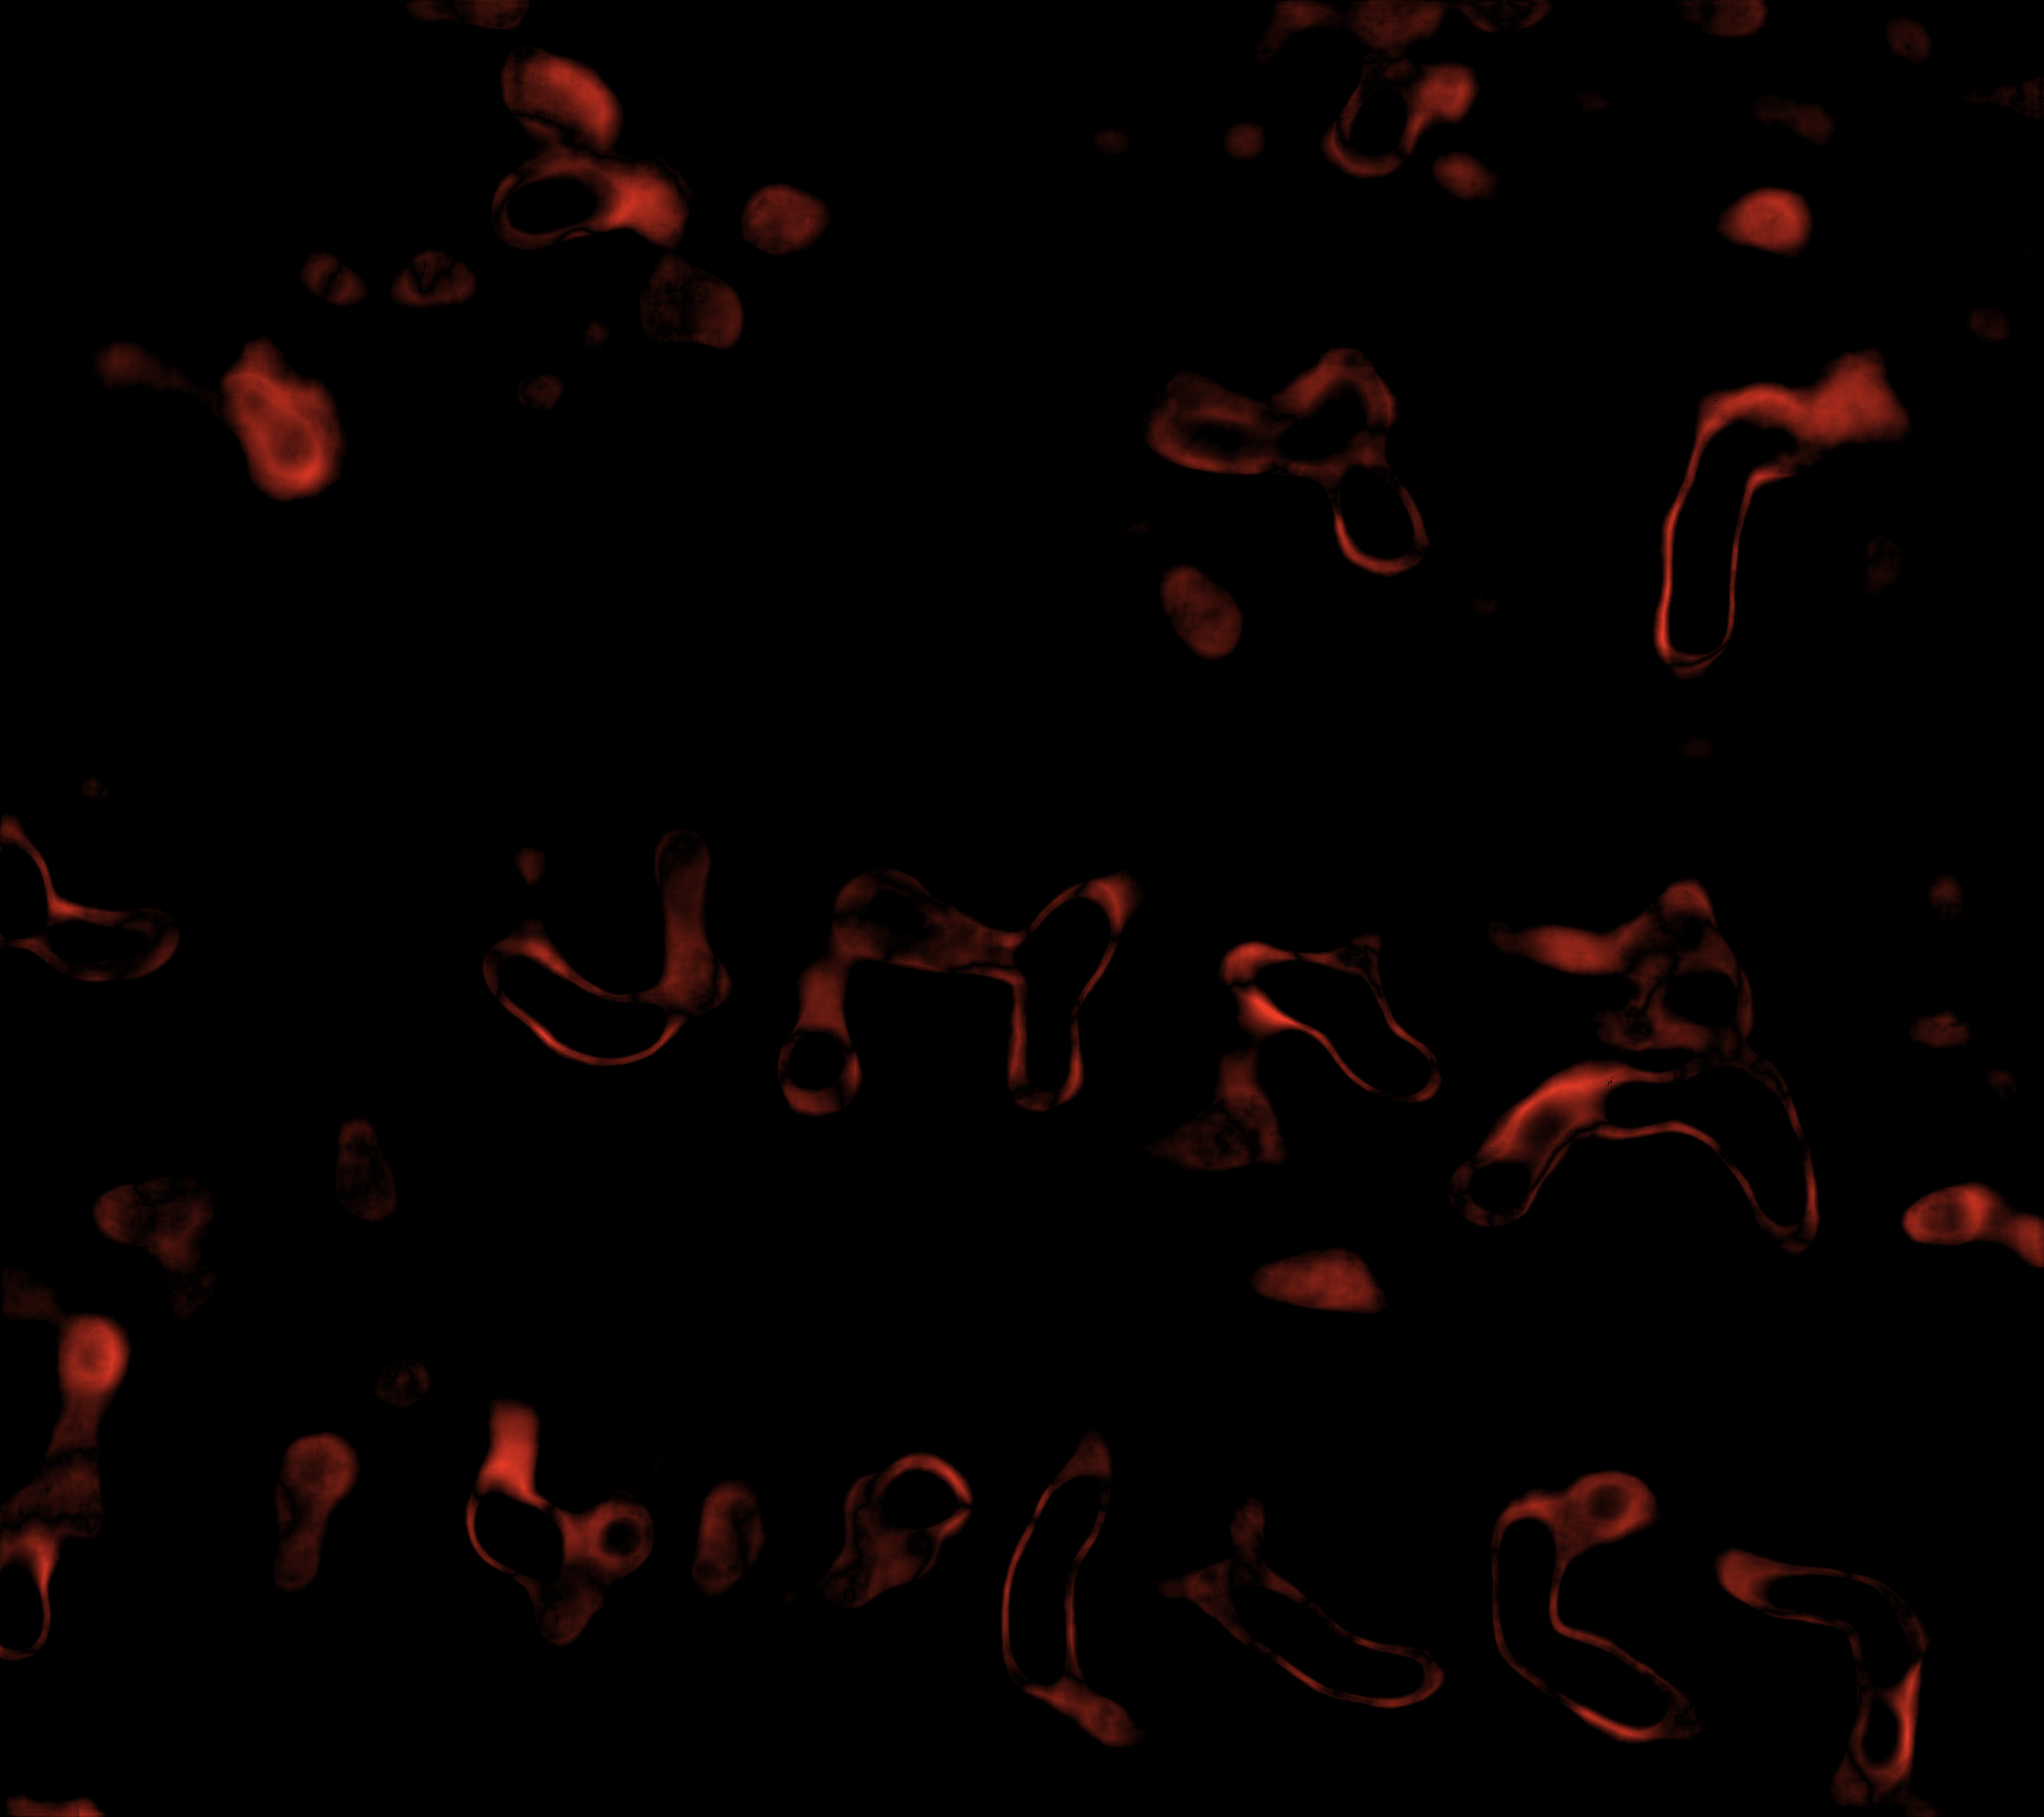
\includegraphics[width=0.29\textwidth]{../figures/m4/ag2_3_difference.png}
\caption{Control unit 0841 ag2. Left, Reader v3 (AUC 0.8297); centre, \MfName{} (AUC 0.8214); right, the red difference between the two maps. Each map is stretched between its own percentiles, the panels are shown at the full resolution of the file.}\label{fig:m4-ag2}
\end{figure*}

\begin{figure*}[!tp]
\centering
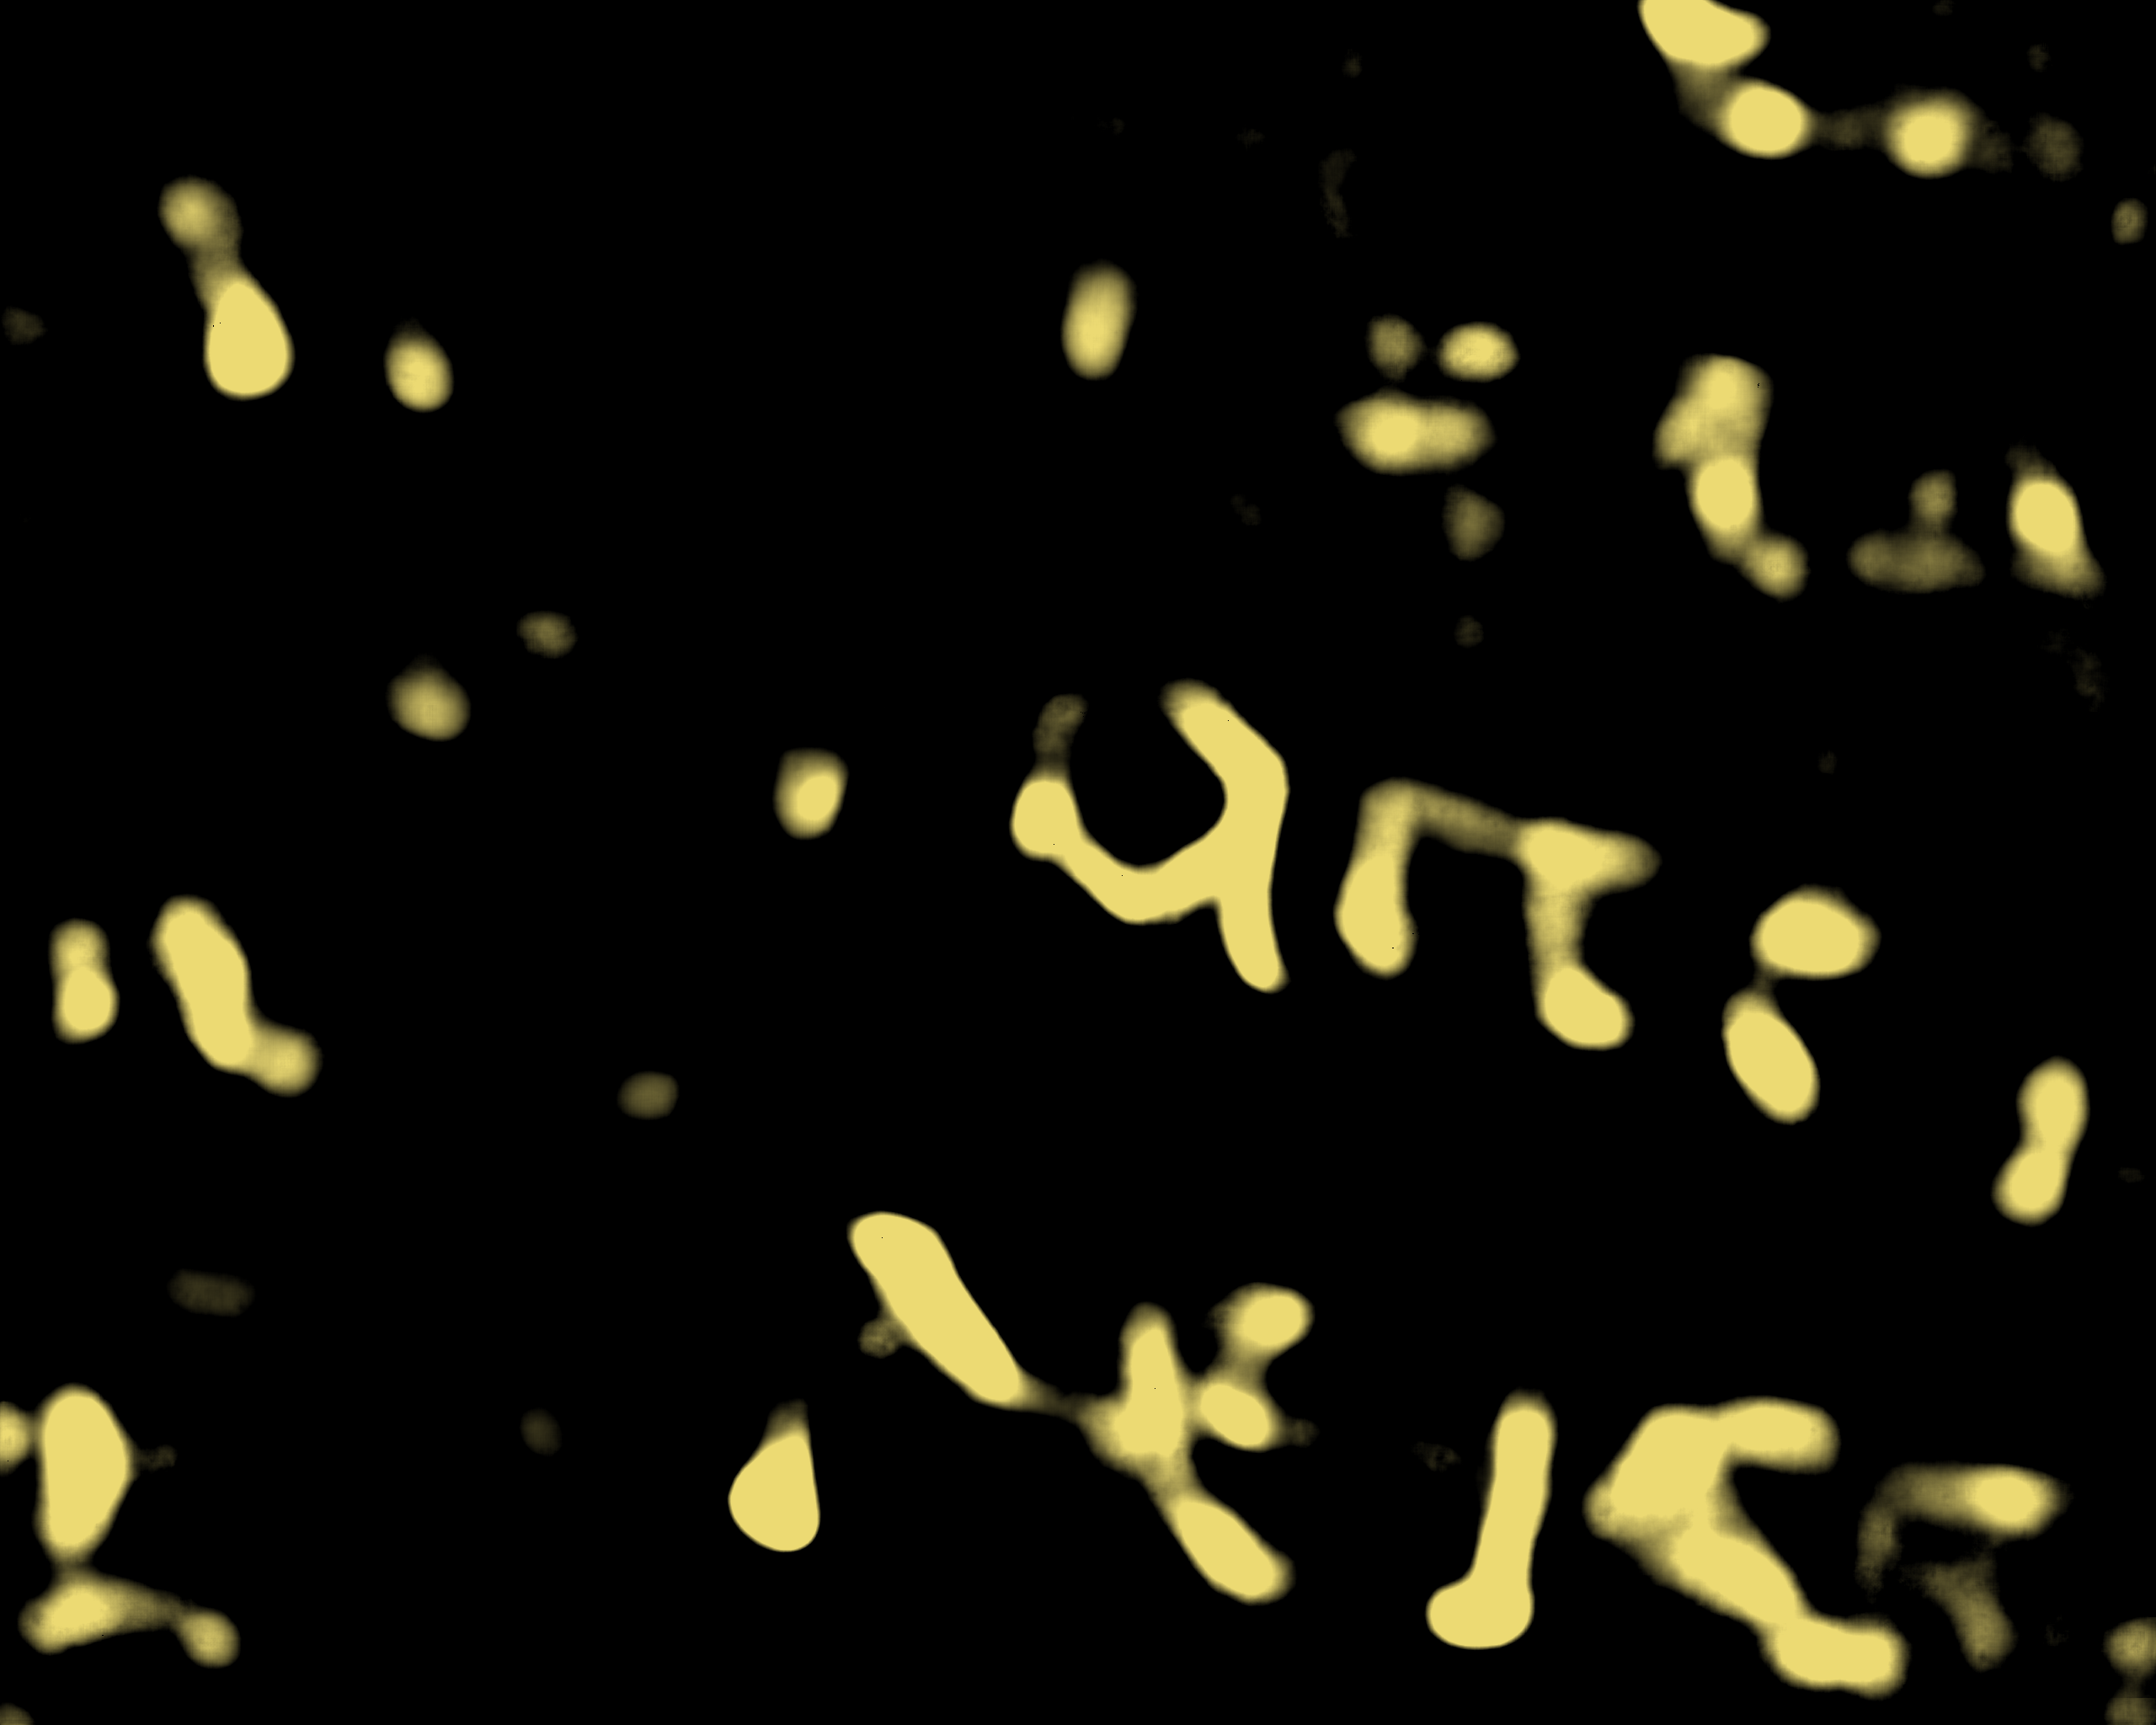
\includegraphics[width=0.29\textwidth]{../figures/m4/w00_1_reader-v3.png}
\hspace{3pt}
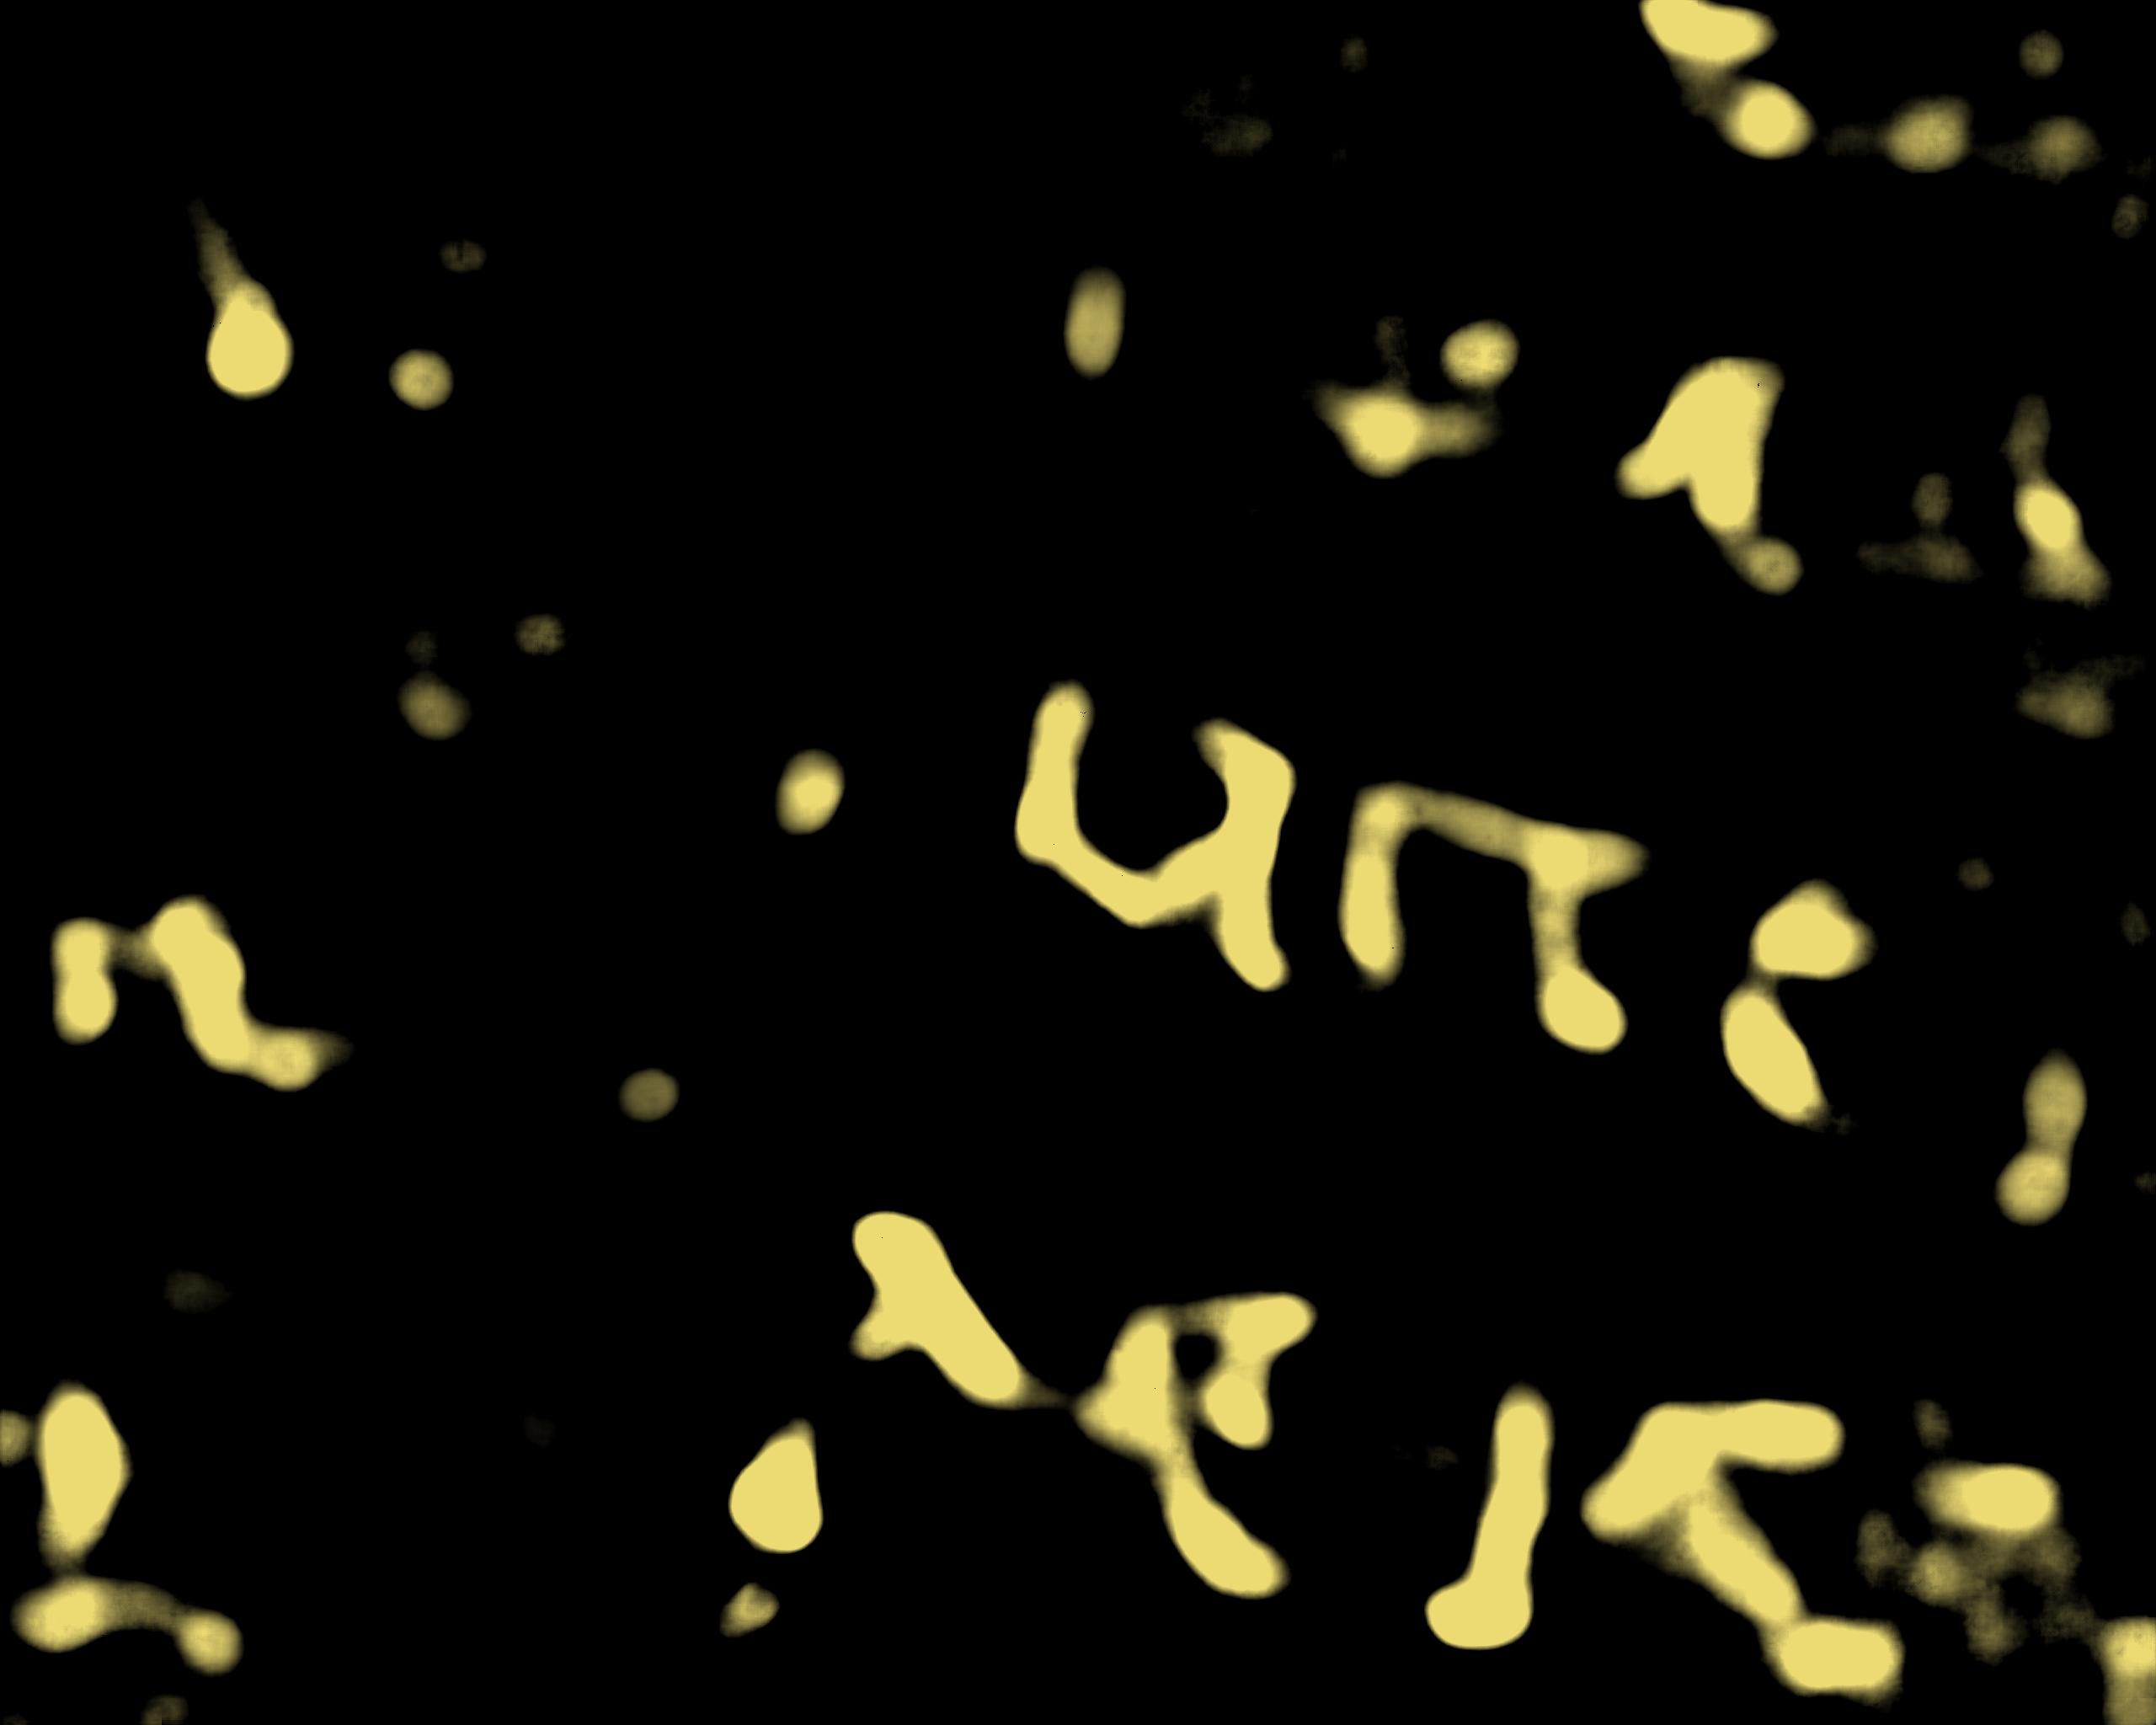
\includegraphics[width=0.29\textwidth]{../figures/m4/w00_2_m4.png}
\hspace{3pt}
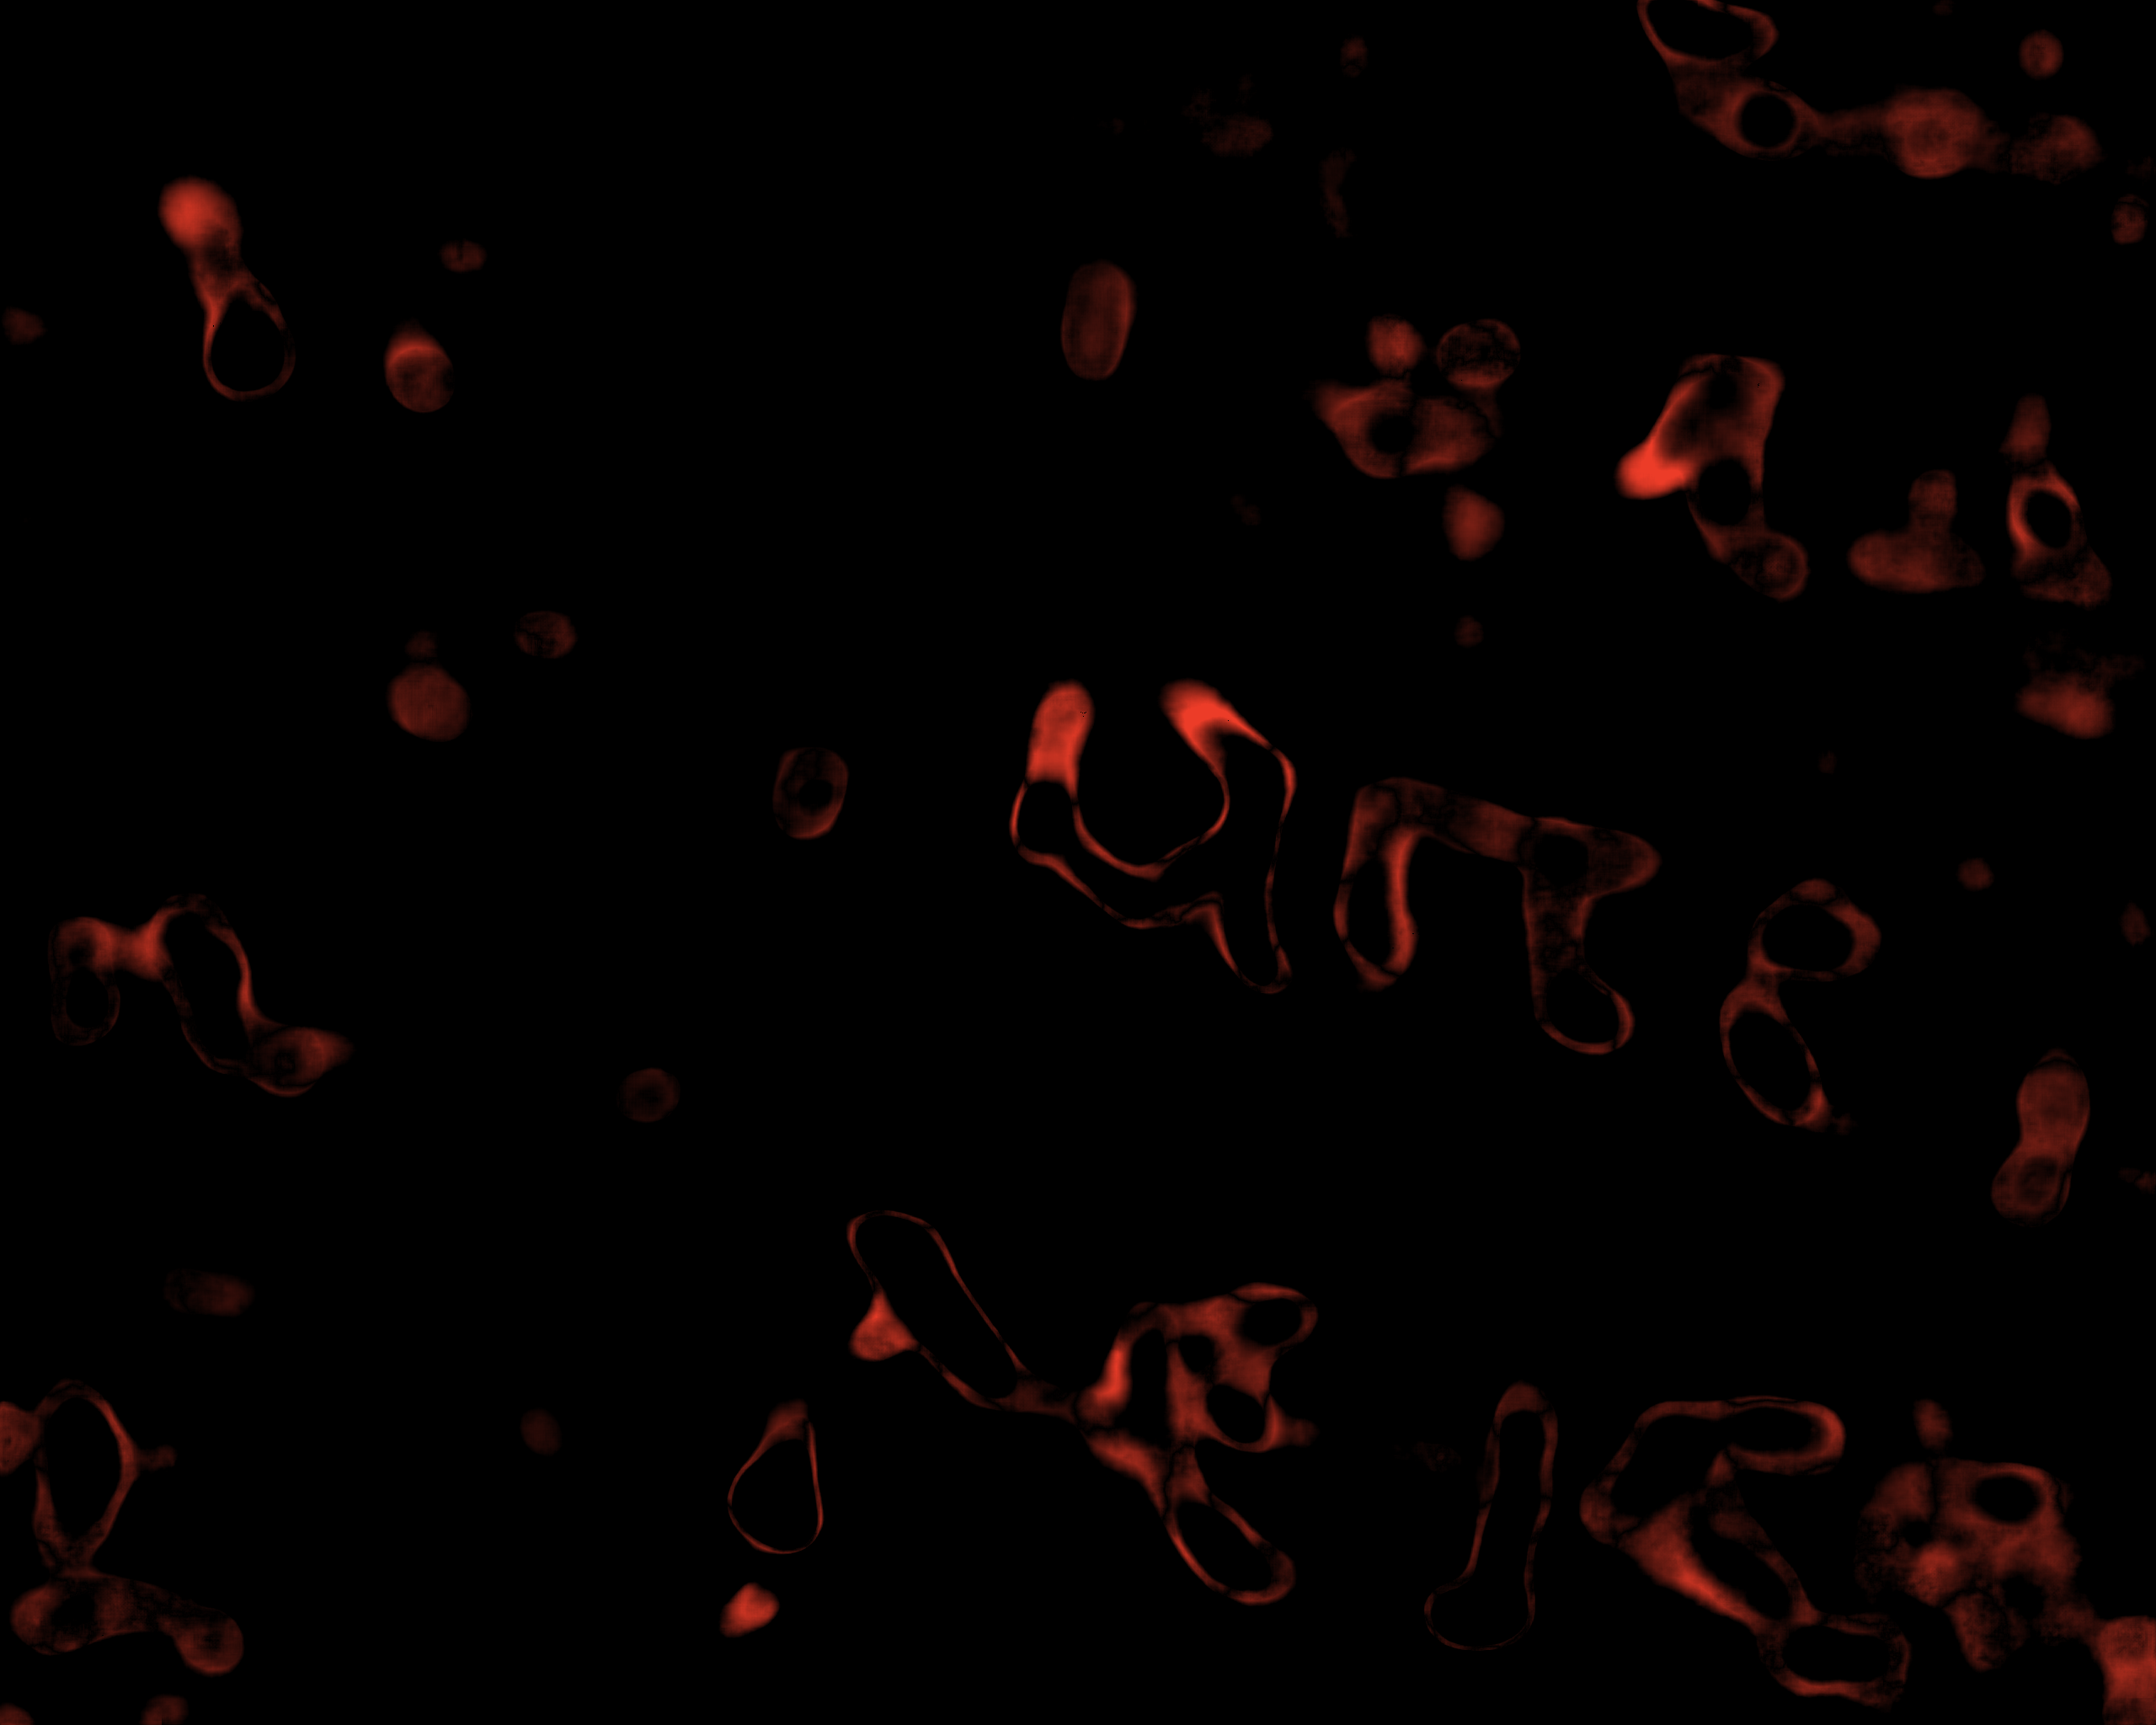
\includegraphics[width=0.29\textwidth]{../figures/m4/w00_3_difference.png}
\caption{Control unit 0841 w00. Left, Reader v3 (AUC 0.9055); centre, \MfName{} (AUC 0.9064); right, the red difference between the two maps. Each map is stretched between its own percentiles, the panels are shown at the full resolution of the file.}\label{fig:m4-w00}
\end{figure*}

\begin{figure*}[!tp]
\centering
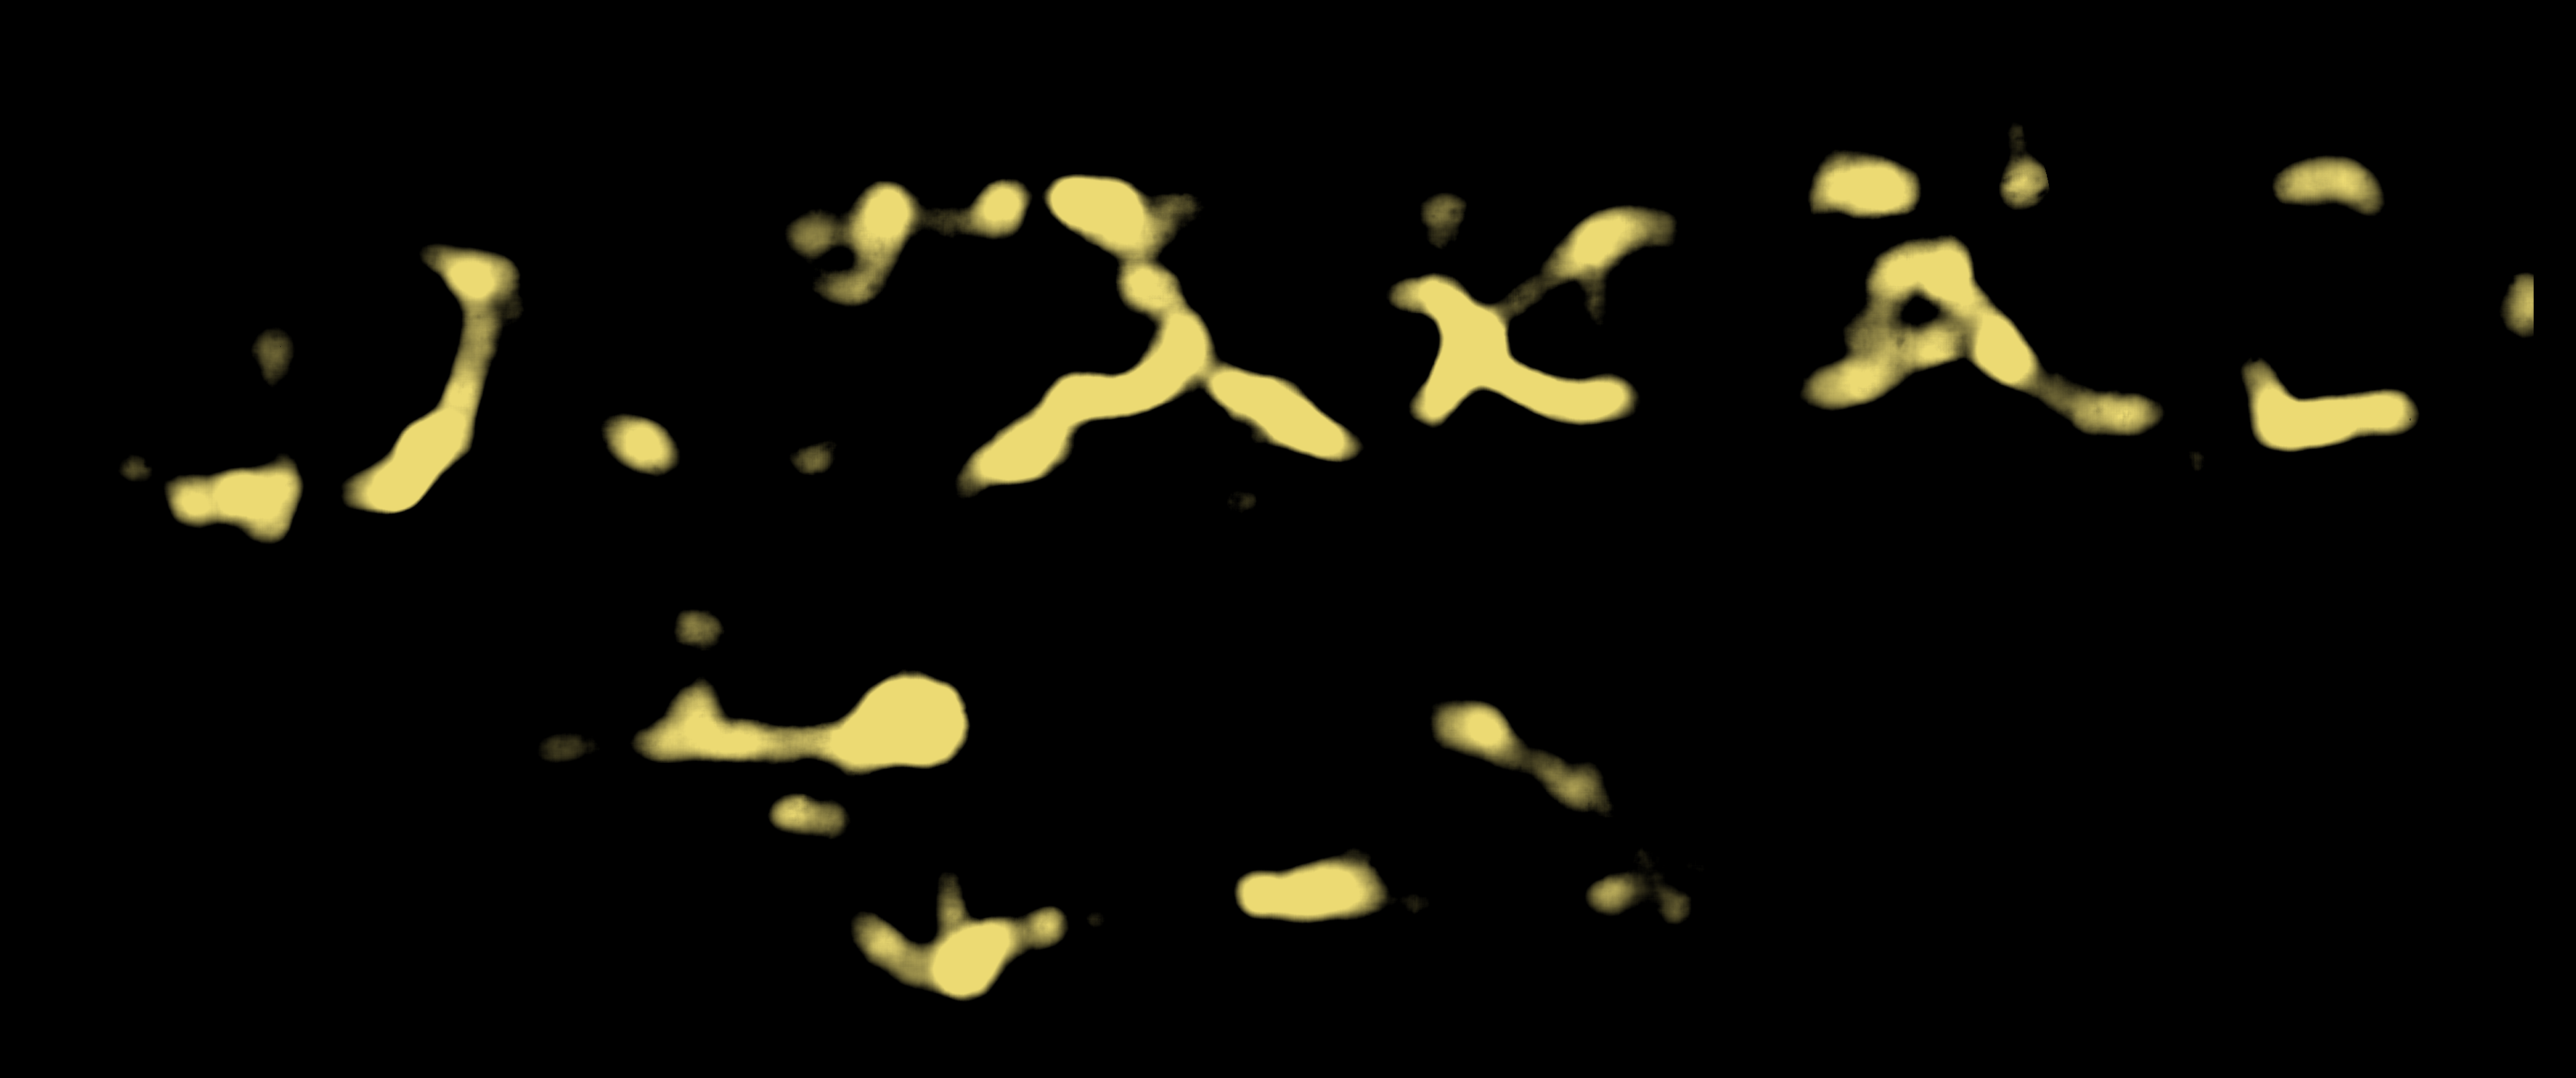
\includegraphics[width=0.29\textwidth]{../figures/m4/w058_1_reader-v3.png}
\hspace{3pt}
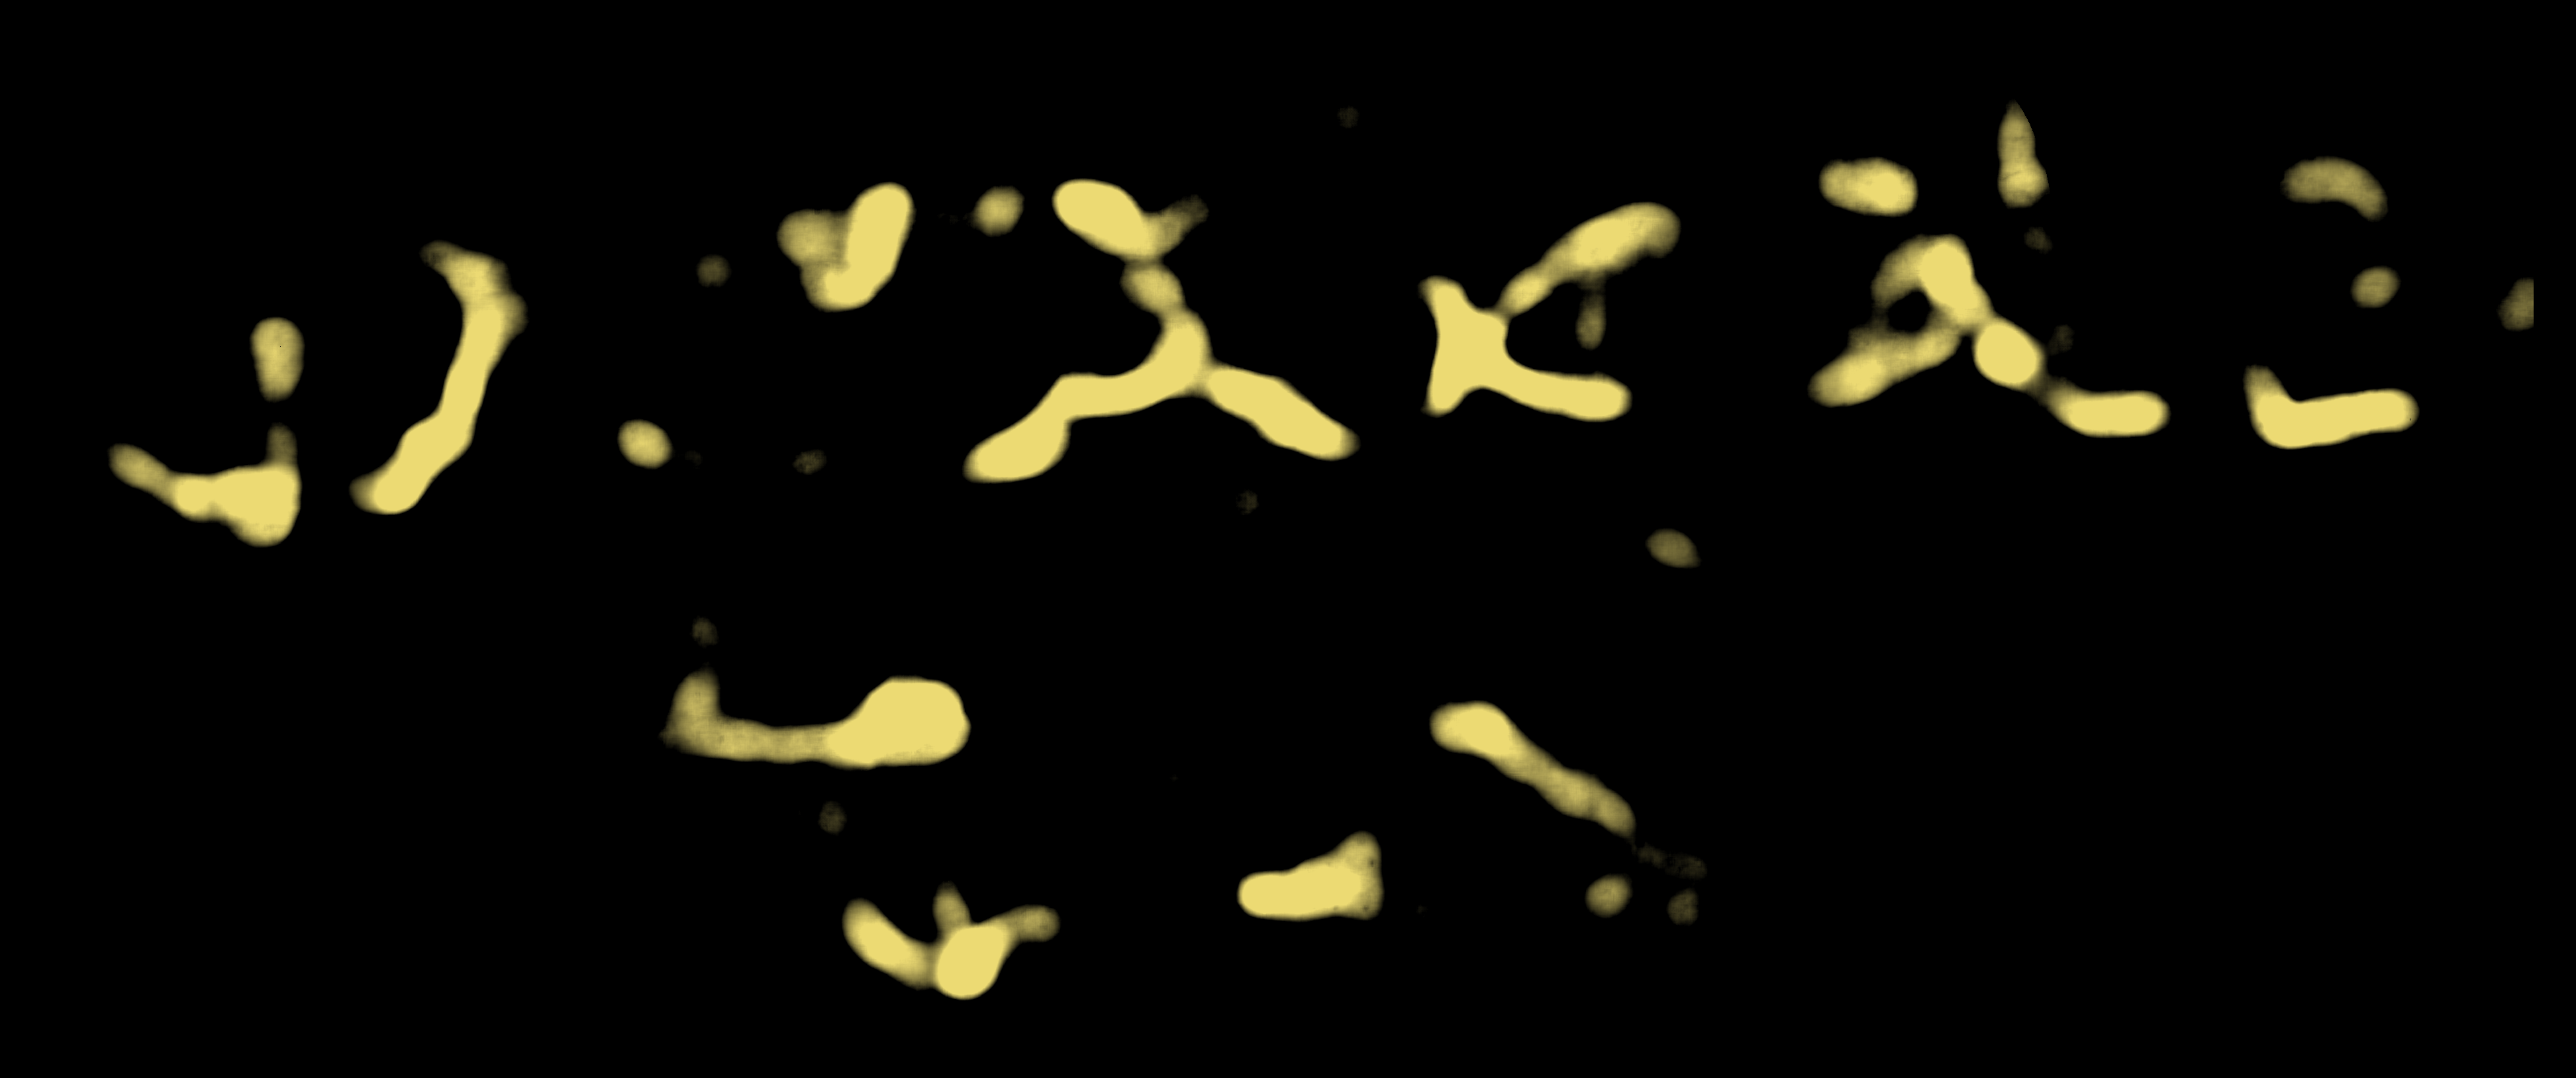
\includegraphics[width=0.29\textwidth]{../figures/m4/w058_2_m4.png}
\hspace{3pt}
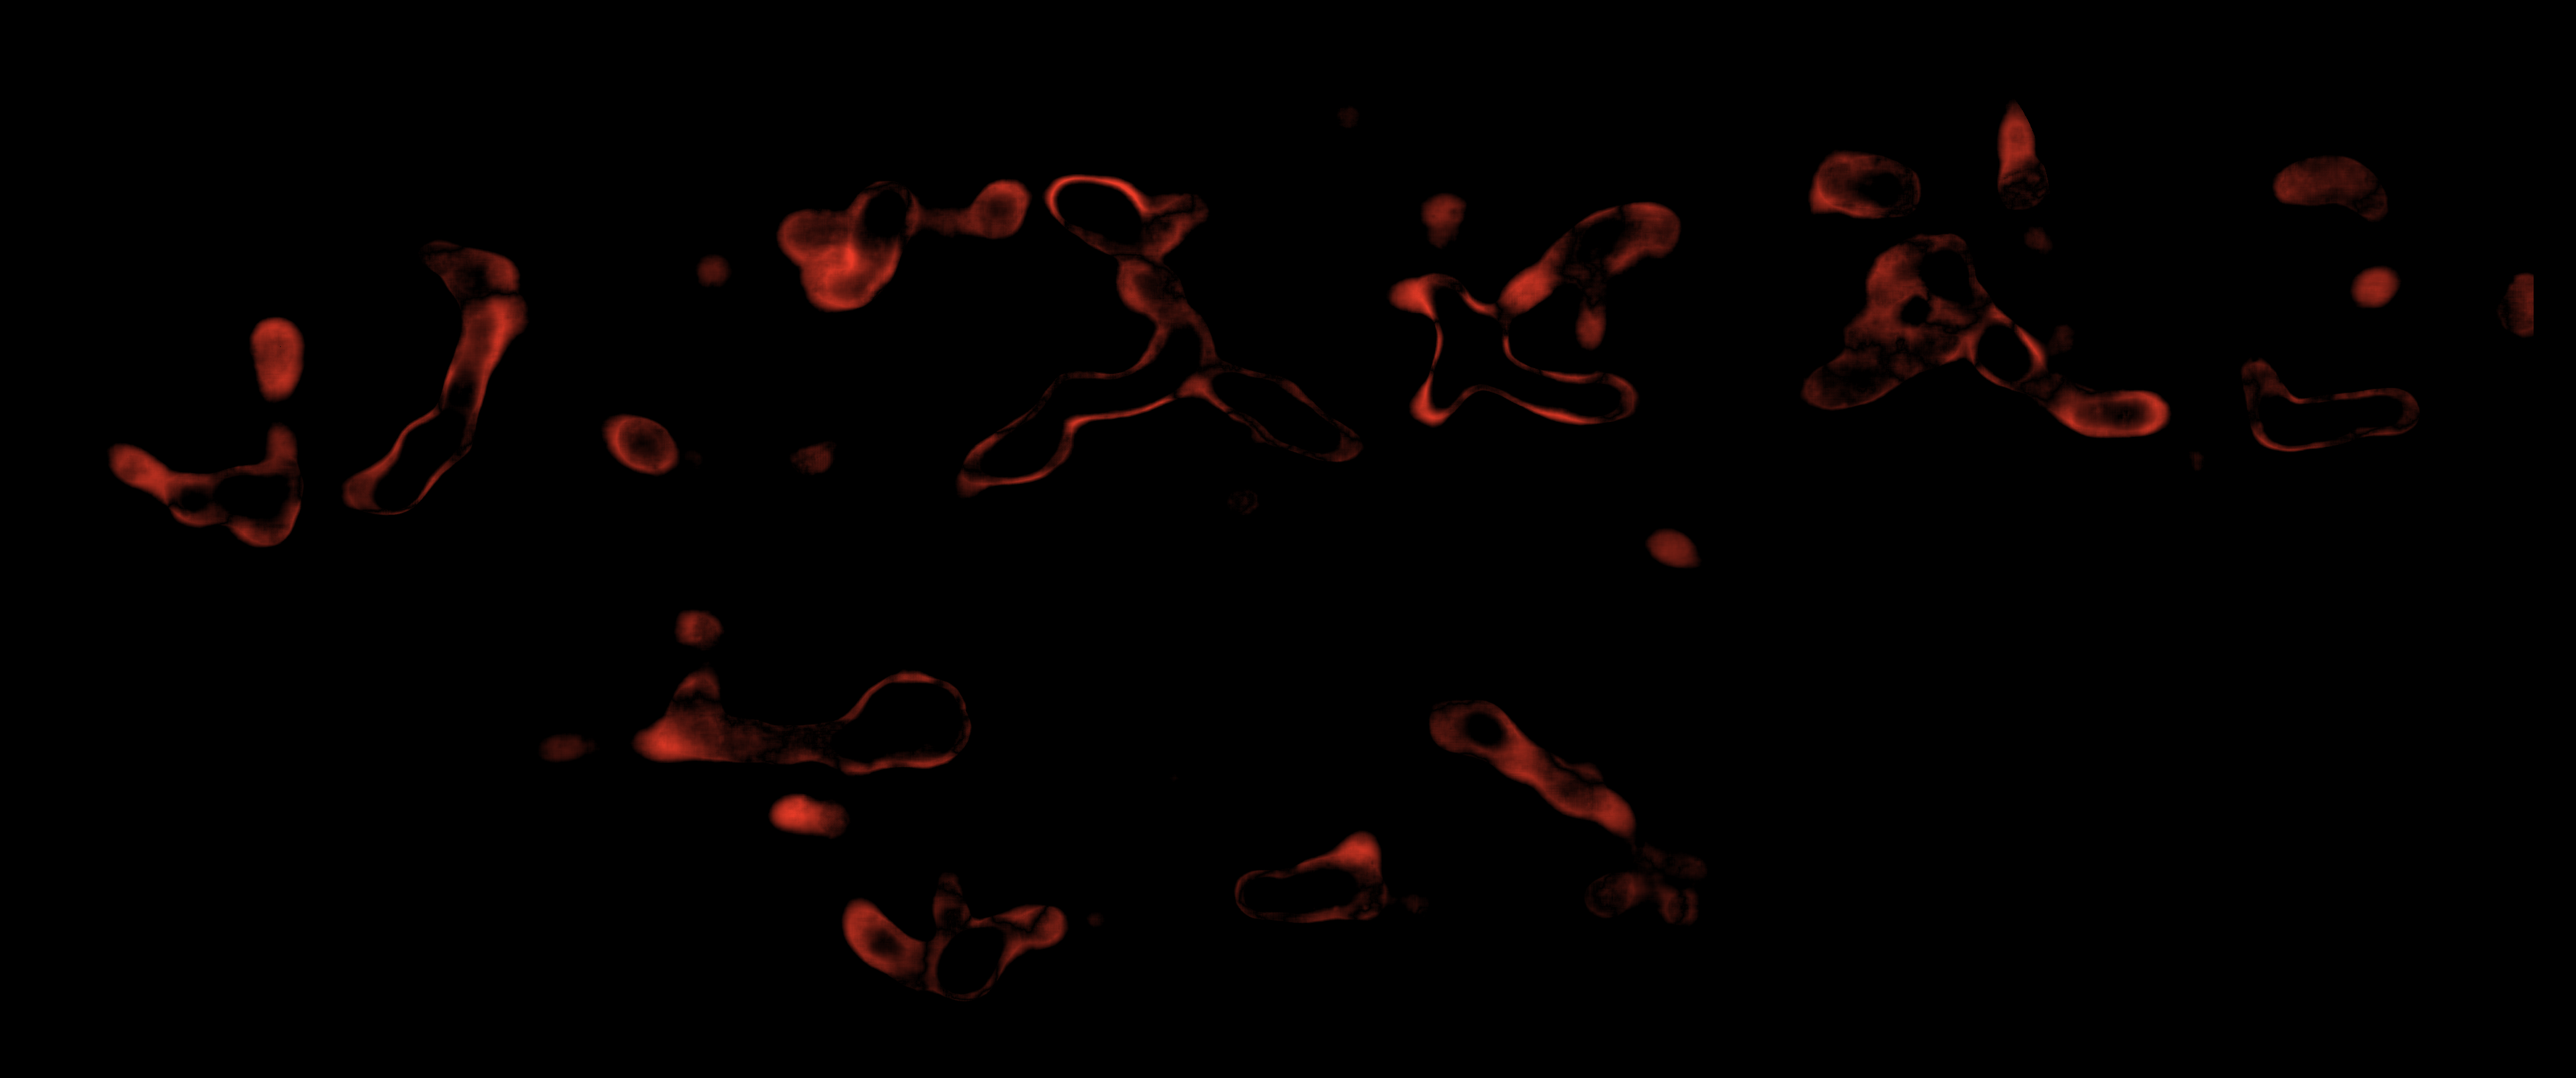
\includegraphics[width=0.29\textwidth]{../figures/m4/w058_3_difference.png}
\caption{Control unit 1447 w058. Left, Reader v3 (AUC 0.8610); centre, \MfName{} (AUC 0.8616); right, the red difference between the two maps. Each map is stretched between its own percentiles, the panels are shown at the full resolution of the file.}\label{fig:m4-w058}
\end{figure*}

\begin{figure*}[!tp]
\centering
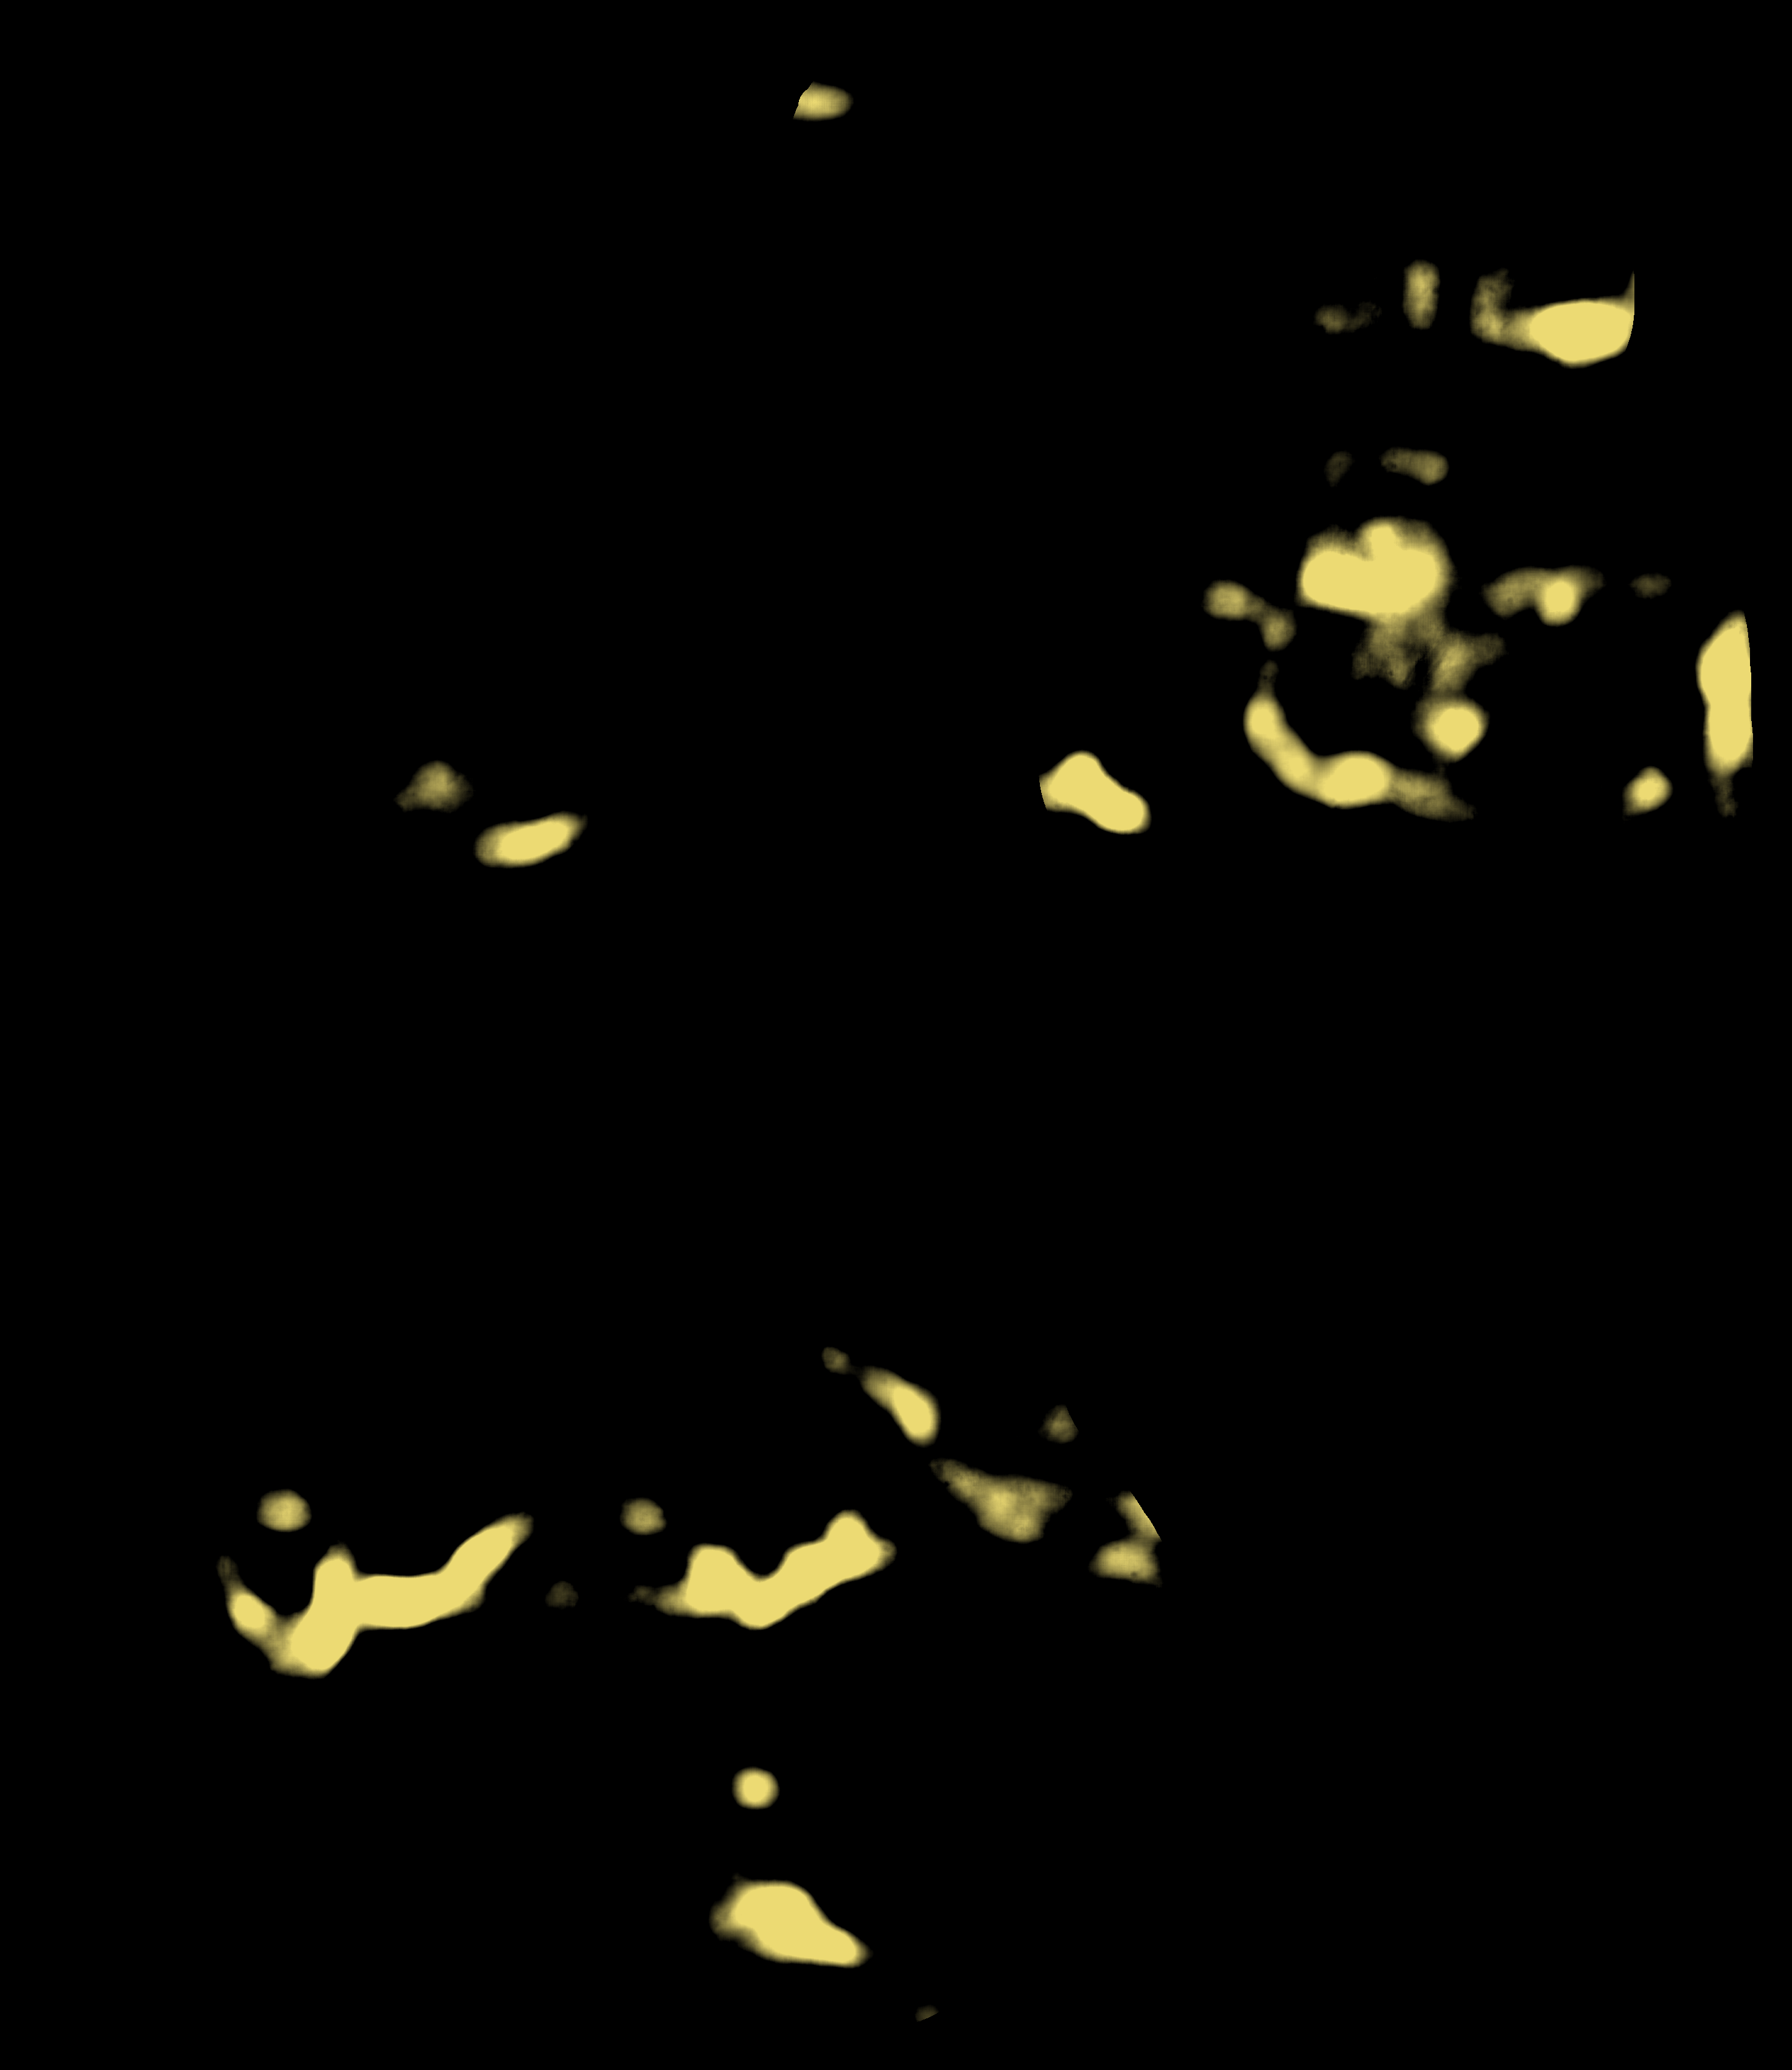
\includegraphics[width=0.29\textwidth]{../figures/m4/w060_1_reader-v3.png}
\hspace{3pt}
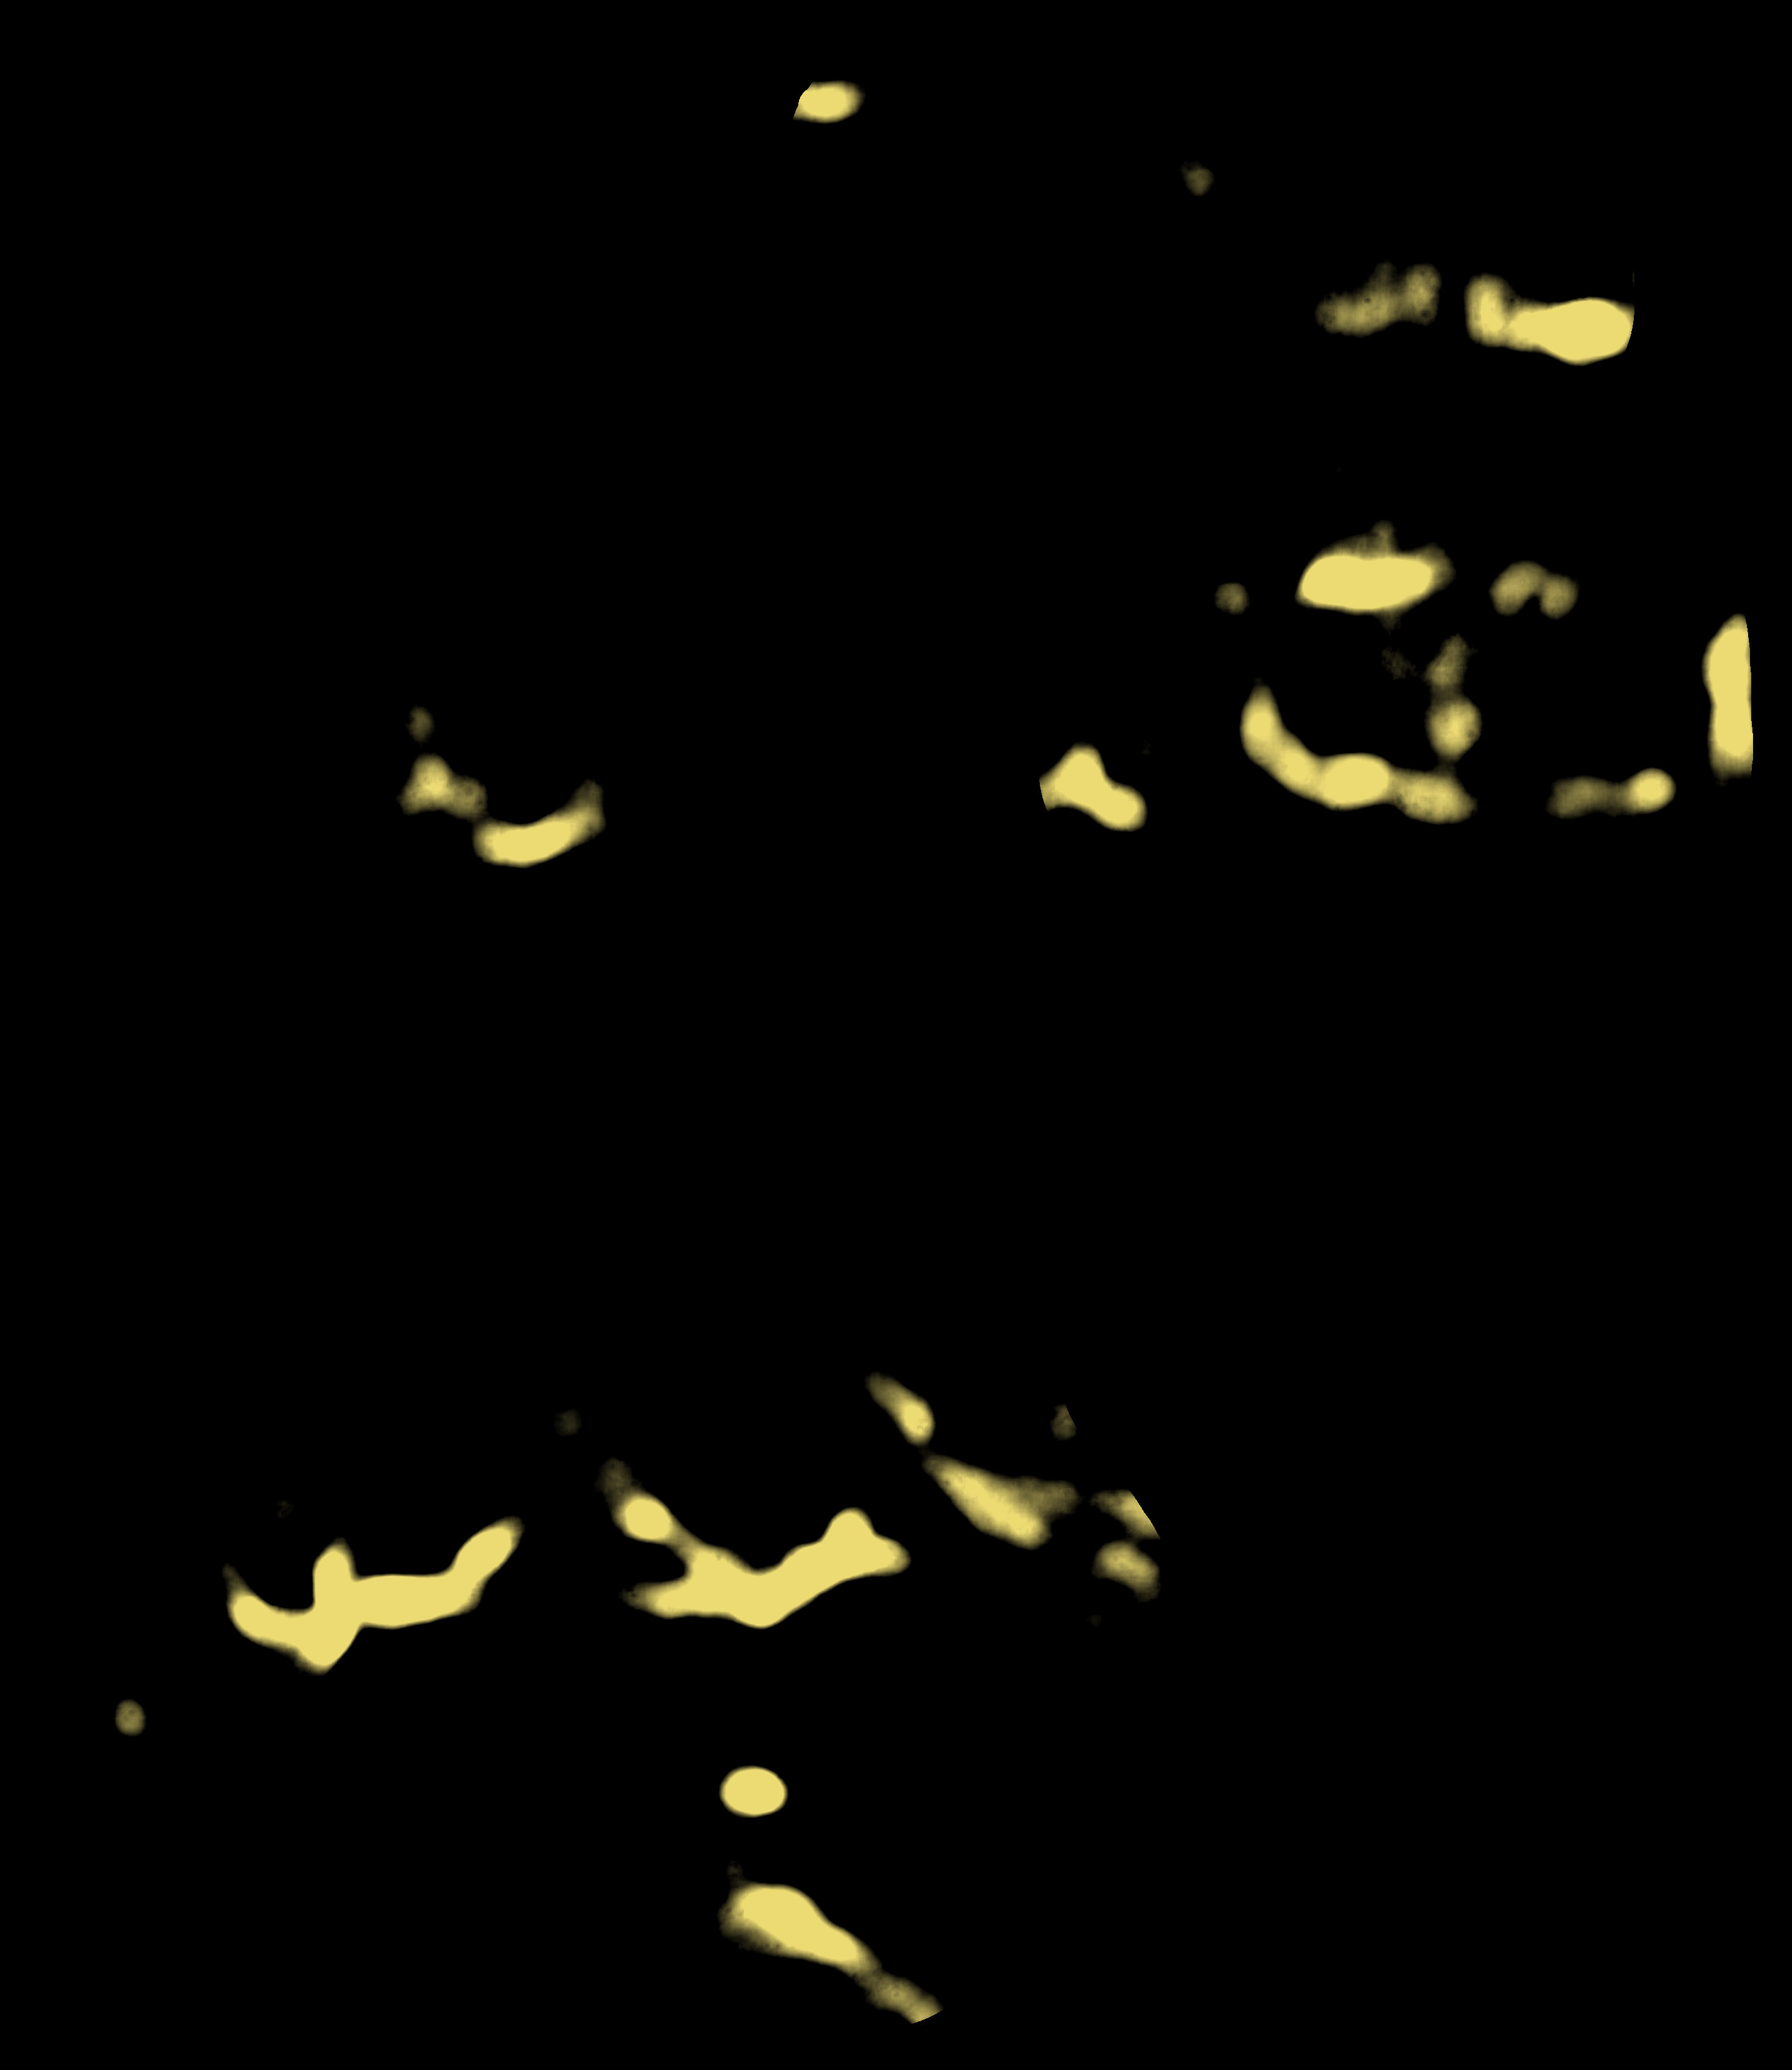
\includegraphics[width=0.29\textwidth]{../figures/m4/w060_2_m4.png}
\hspace{3pt}
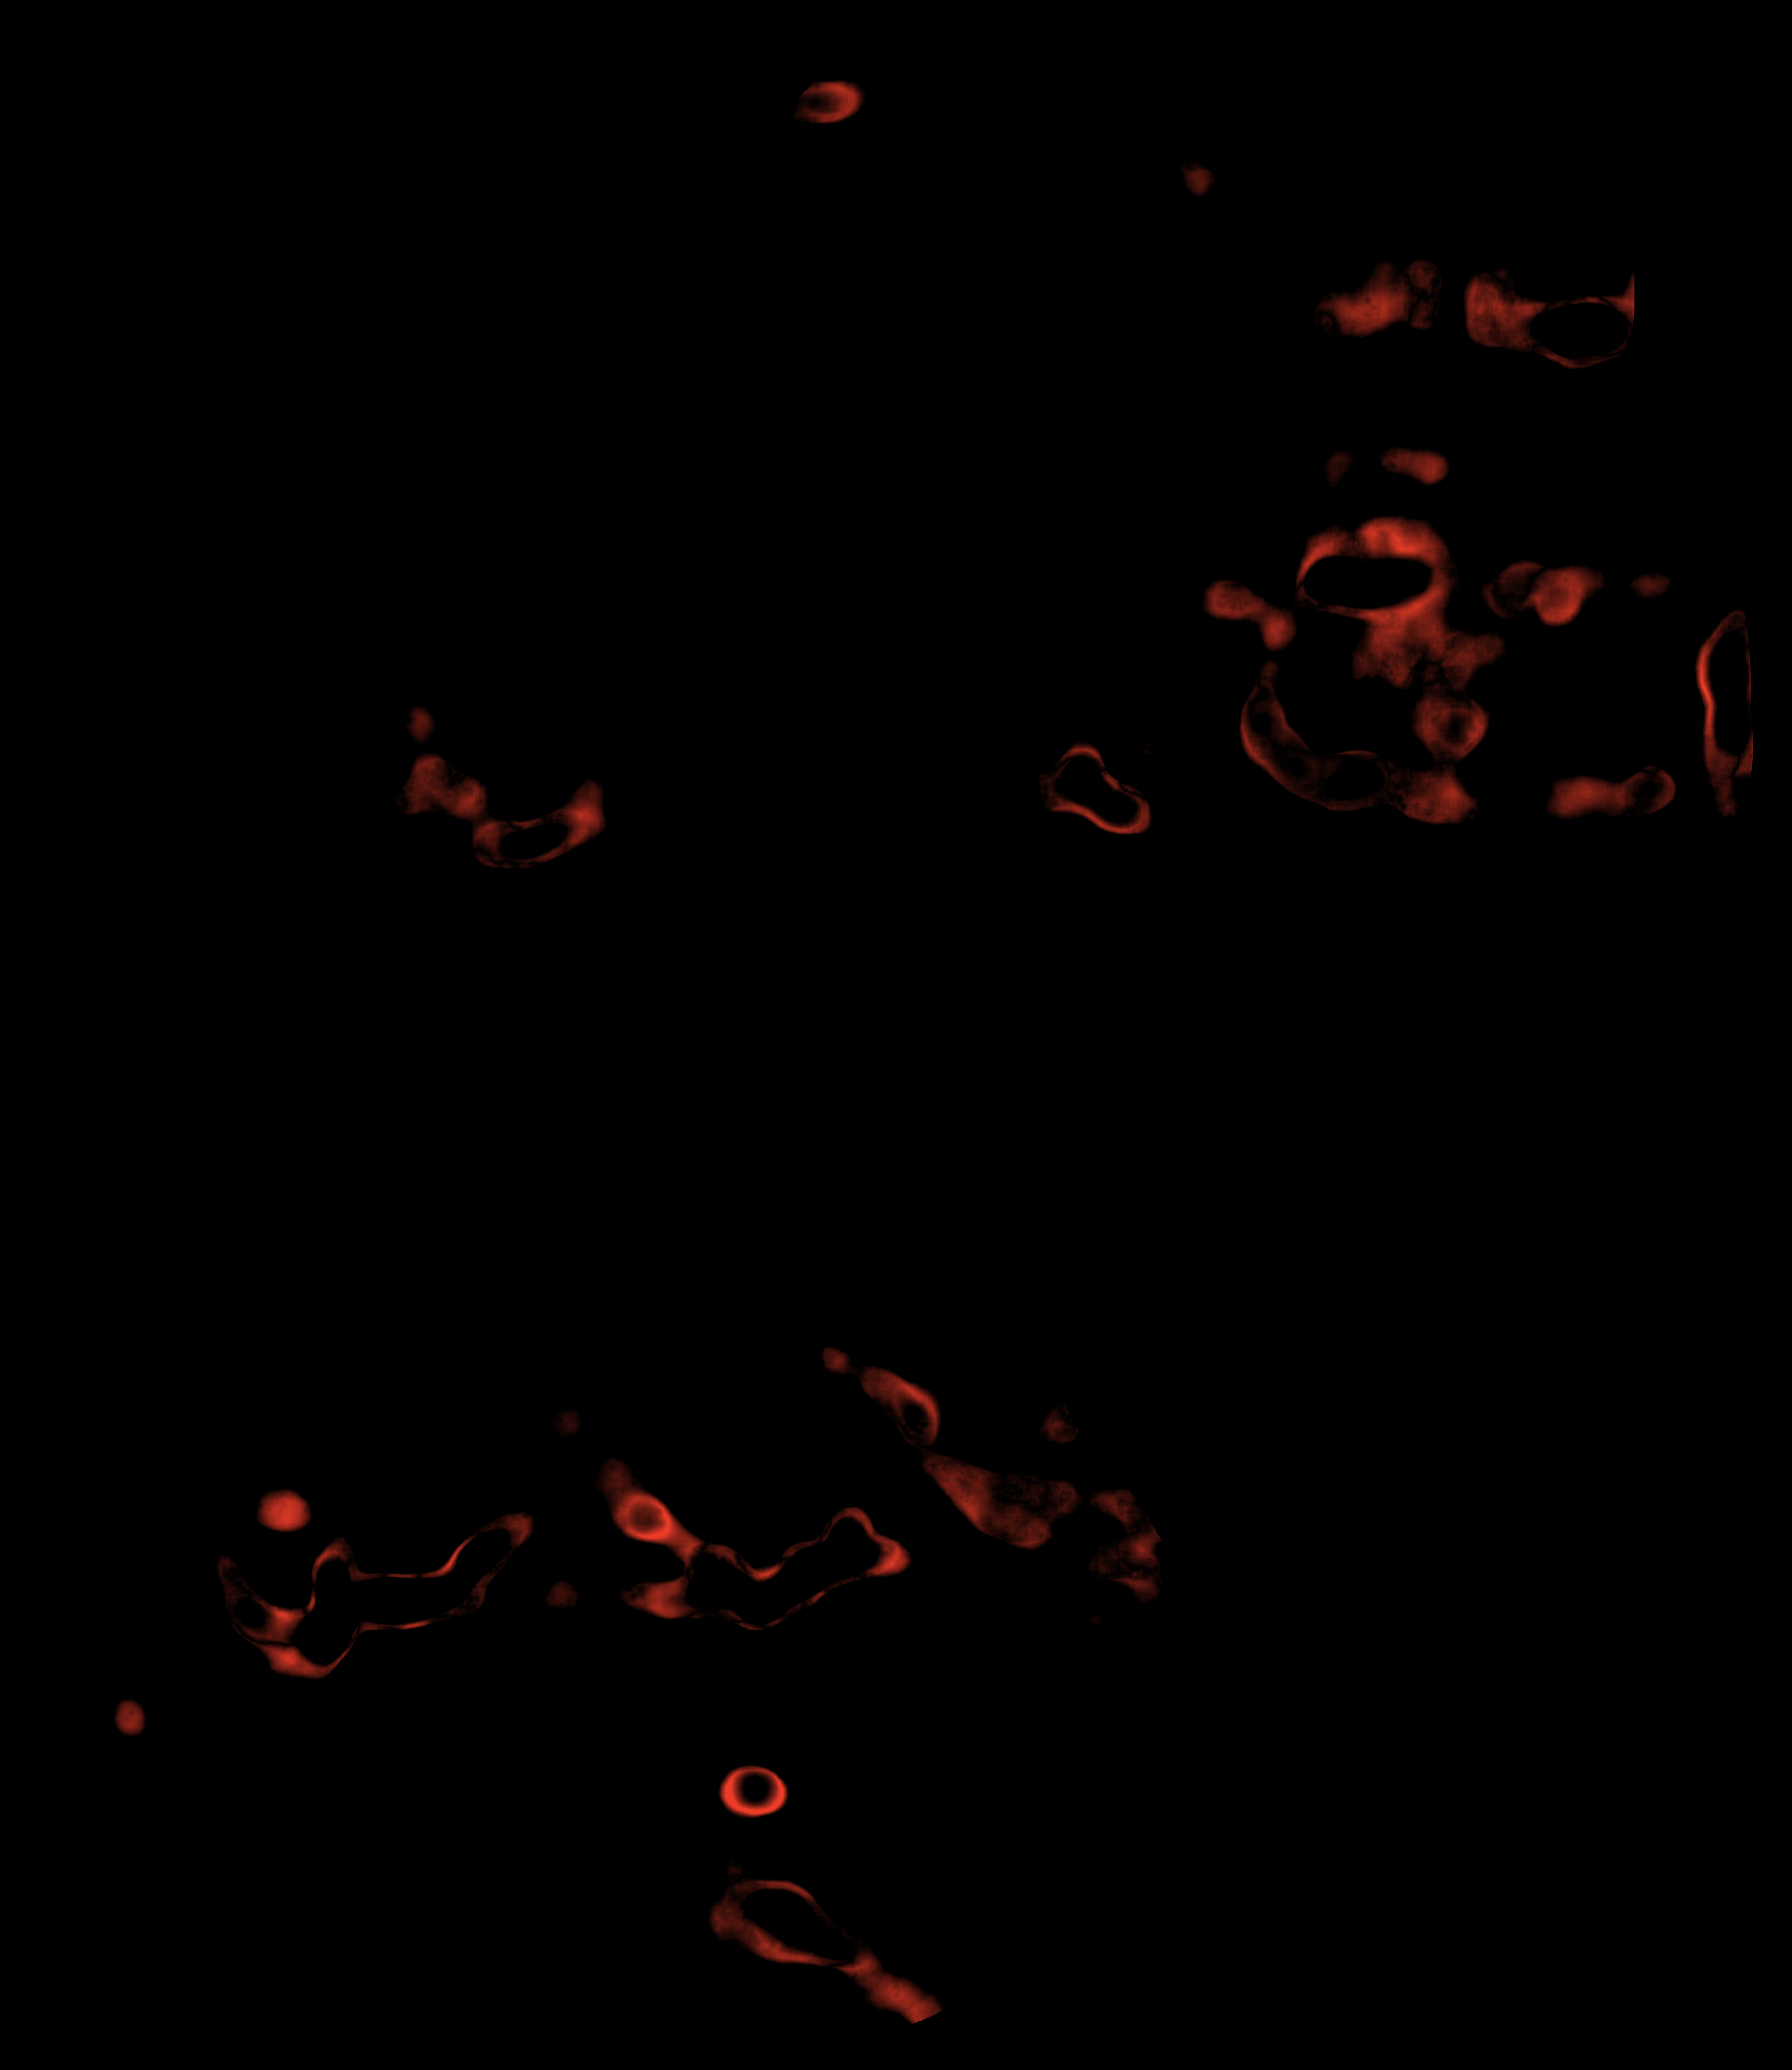
\includegraphics[width=0.29\textwidth]{../figures/m4/w060_3_difference.png}
\caption{Control unit 1447 w060. Left, Reader v3 (AUC 0.7842); centre, \MfName{} (AUC 0.7900); right, the red difference between the two maps. Each map is stretched between its own percentiles, the panels are shown at the full resolution of the file.}\label{fig:m4-w060}
\end{figure*}
